\documentclass{report}

\usepackage{amsmath}
\usepackage[inlinechap]{settings/fncystyle}
\input{preamble}
\input{macros}
\input{letterfonts}

\usepackage[indent=0pt]{parskip}

\renewcommand{\chaptername}{Capitolo}
\renewcommand{\contentsname}{Indice}

\title{\Huge{Appunti Elettrodinamica}}
\author{Giacomo Galliani, corso del prof. N. Piovella}
\date{Anno accademico 2025-2026}

\begin{document}

\maketitle
\newpage% or \cleardoublepage
% \pdfbookmark[<level>]{<title>}{<dest>}
\pdfbookmark[section]{\contentsname}{toc}
\tableofcontents
\pagebreak

\chapter{Equazioni di Maxwell}

Le eq. di Maxwell sono 8 eq. scalari per 4 campi vettoriali, $B, E, D, H$, e sono date da 

\begin{align}
    & \nabla \cdot B = 0 \\
    & \underbrace{\nabla \times E = -\partial_t B}_{eq. omogenee} \\
    & \nabla \cdot D = \rho \\
    & \underbrace{\nabla \times H = J + \partial_t D}_{eq. in-omogenee}
\end{align}

I campi $D, H$ sono legati ai campi $E, B$ in base alla presenza o meno di materiali, in particolare si ha \emph{nel vuoto}
\begin{align}
    & D = \epsilon_0 E \\
    & H = B /\mu_0
\end{align}
Invece in presenza di materiali \emph{macroscopici}, si ha
\begin{align}
    & D = \epsilon_0 E + P \\
    & H = B /\mu_0 - M
\end{align}

Le costanti sono date da $\epsilon_0 = 8.85 \cdot 10^{-12}F m^{-1},  \quad \mu_{0} = 4\pi \cdot 10^{-7} Hm^{-1}$. 

Chiaramente, le quanità fondamentali sono i campi $E, B$, mentre i campi $D, H$ sono campi ausiliari che permettono di ottenere delle buone approssimazioni senza contare tutti i contributi ai campi delle cariche legate che formano la materia ordinaria. \\

Le eq. di Maxwell sono coerenti con l'eq. di continuità, che a sua volta implica la conservazione della carica. Infatti, ricordato che per ogni campo vettoriale $A$, vale $\nabla \cdot (\nabla \times A ) = 0$, ponendoci nel vuoto e applicando la divergenza all'eq. , troviamo 

\begin{equation}
    0 = \mu_0(\nabla \cdot J + \epsilon_0 \partial_t (\nabla \cdot E)) = \mu_o(\nabla \cdot J + \partial_t \rho )
\end{equation}

Vediamo dunque che la coerenza è assicurata grazie alla \emph{corrente di spostamento} inserita da Maxwell. La più importante conseguenza dell'aggiunta di questo termine è certamente la predizione teorica delle onde elettromagnetiche: Se ci poniamo infatti nel vuoto, in assenza di cariche, e applichiamo il rotore alla legge di Faradat otteniamo: 

\begin{equation}
    \nabla \times \nabla \times E = \nabla(\nabla \cdot E) - \nabla^2E = - \nabla^2E = - \frac{\partial}{\partial t}(\nabla \times B) = - \epsilon_0 \mu_0 \frac{\partial^2}{\partial t^2}E
\end{equation}

Abbiamo dunque ottenuto l'eq. delle onde: 

\begin{tcolorbox}[colback=doc!15, colframe=black, boxrule=1pt]
\begin{equation}
    \left(\frac{1}{c^2}\frac{\partial^2}{\partial t^2} - \nabla^2 \right)E = 0
\end{equation}
\end{tcolorbox}

Con gli stessi passaggi, avemmo anche potuto ottenere 

\begin{tcolorbox}[colback=doc!15, colframe=black, boxrule=1pt]
\begin{equation}
    \square B = 0 
\end{equation}
\end{tcolorbox}

Dove abbiamo definito l'operatore D'Alembertiano $\square = \left(\frac{1}{c^2}\frac{\partial^2}{\partial t^2} - \nabla^2 \right)$. \\

Una volta risolte le eq. per una data distribuzione di carica e corrente $\rho, \, J$, la forza agente su una particella "test", di carica $q$ e velocità $v$ è data da 

\begin{equation}
    F = q(E + v \times B)
\end{equation}

\section{Potenziali Elettrodinamici}
Veniamo ora a parlare dei potenziali elettrodinamici: il fatto che il campo $B$ abbia divergenza zero, vuol dire che può essere espresso come il rotore di un altro campo (il \emph{potenziale vettore}), $A$. \\

D'altra parte, la legge di Faraday ci dice che 

\begin{equation}
    \nabla \times E + \partial_t B = \nabla \times (E + \partial_tA) = 0
\end{equation}

Ovvero il campo $E + \partial_tA$ è irrotazionale, e come tale può essere espresso come il gradiente di una funzione scalare, $\phi$. Abbiamo quindi ricavato i campi $E, B$ in termini dei loro potenziali


\begin{equation}
    \label{vector_potential}
     B = \nabla \times A \\
\end{equation}

\begin{equation}
    \label{scalar_potential}
    E = -\nabla\phi - \partial_tA
\end{equation}

Invece, le eq. inomogenee possono essere convertite nelle eq. differenziali per i campi. 

\nt{Le equazioni inomogenee sono scritte in termini dei campi ausiliari \(\vec{H}, \vec{D}\). Per poter scrivere delle equazioni per i potenziali \(\phi, \vec{A}\), la strategia sarà  di scrivere le equazioni in termini di \(\vec{E}, \vec{B}\), e successivamente sostituire per i potenziali usando le relazioni appena determinate.}

\begin{equation}
    \nabla \cdot E = \frac{1}{\epsilon_0}(\rho - \nabla \cdot P) = \frac{\rho_1}{\epsilon_0}
\end{equation}

\begin{equation}
    \nabla \times B = \mu_0(J + \nabla \times M) + \mu_0\epsilon_0\partial_tE = \mu_0J_1 + \frac{1}{c^2}\partial_tE
\end{equation}

Ora posso sostituire i potenziali usando le eq. \ref{vector_potential}, \ref{scalar_potential}, e otteniamo:

\begin{equation}
    \nabla \cdot (-\nabla\phi - \partial_tA) = \frac{\rho_1}{\epsilon_0} \rightarrow \nabla^2\phi + \partial_t(\nabla \cdot A) = -\frac{\rho_1}{\epsilon_0}
\end{equation}

ed inoltre 

\begin{align}
    &\nabla \times (\nabla \times A) - \frac{1}{c^2}(-\nabla\partial_t\phi - \partial_{tt}A) = \mu_0 J_1 \\
    &\nabla(\nabla \cdot A) - \nabla^2A + \frac{1}{c^2}\nabla\partial_t\phi +\frac{1}{c^2} \partial_{tt}A = \mu_0 J_1 \\
    & \square A + \nabla(\nabla \cdot A + \frac{1}{c^2}\partial_t\phi) = \mu_0J_1
\end{align}

Così scritte, le eq. sono difficili da risolvere, soprattutto perchè sono equazioni accoppiate. Ci chiediamo se esista un modo disaccopiarle. Questo modo è l'invarianza di gauge: Considero infatti la seguente trasformazione sui potenziali elettromagnetici: 

\[\begin{cases}
    A^{'} = A + \nabla\chi \\
    \phi^{'} = \phi - \partial_t\chi
\end{cases}\]

A partire da questi, i nuovi campi $E^{'}, B^{'}$ saranno dati da: 

\[\begin{cases}
    B^{'} = \nabla \times (A + \nabla \chi) = \nabla \times A = B \\
    E^{'} = -\nabla(\phi - \partial_t\chi) - \partial_t(A + \nabla\chi) = -\nabla \phi -\partial_tA = E
\end{cases}\]

Dunque abbiamo la libertà di agire sui potenziali con una trasformazione di gauge quando vogliamo, e questo non cambierà i campi $E, B$. 

\subsection{gauge di Lorentz}

Al fine di disaccopiare le eq. per i potenziali, provo a vedere se esiste una trasformazione di gauge t.c. valga $\nabla \cdot A + \frac{1}{c^2}\partial_t\phi =0$. 

Se esiste, la funzione $\chi$ deve soddisfare

\begin{align}   
    &0  = \nabla \cdot A^{'} + \frac{1}{c^2}\partial_t\phi^{'} = \nabla \cdot (A + \nabla \chi) + \frac{1}{c^2}(\partial_t\phi - \partial_{tt}\chi) \\
    &0 = \square\chi + \nabla\cdot A + \frac{1}{c^2}\partial_t\phi
\end{align}

Questo è sufficente a mostrare che $\chi$ esiste. Questo gauge è detto gauge di Lorentz. In questo gauge, le eq. per i campi diventano nella forma 

\[\begin{cases}
    \square A = \mu_0J_1 \\
    \square \phi = \frac{\rho_1}{\epsilon_0}
\end{cases}\]

Il motivo del nome è chiaro: trattando allo stesso modo $\phi, A$ la trattazzione è manifestamente covariante. \\

\subsection{gauge di Coulomb}

Una altra possibile scelta è il gauge di Coulomb, dove $\nabla \cdot A = 0$. Si noti che anche questa condizione è ottenibile tramite una trasformazione di gauge, infatti basta scegliere $\nabla^2\chi = - \nabla \cdot A \rightarrow \nabla \cdot A^{'} =0$. La comodità di questo è che si conserva l'eq. di Poisson: 

\[\begin{cases}
    \nabla^2\phi = -\frac{\rho_1}{\epsilon_0} \\
    \square A = \mu_0J_1 - \frac{1}{c^2}\partial_t(\nabla\phi)
\end{cases}\]

Nonostante questo sembra non rispettare la casualità, bisogna ricordare che i veri oggetti fisici sono i campi $E, B$ e svolgendo i conti dettagliati è possibile mostrare che questi rispettano la casualità. 

Spesso, la quantità $J_T = J_1 - \epsilon_o\partial_t(\nabla\phi)$, è detta \emph{corrente trasversa}. Infatti, il teorema di Hermoltz dice che, dato un campo vettoriale $G(x)$, è sempre possibile scomporlo in 

\begin{equation}
    G(x) = G_{||}(x) + G_{T}(x)
\end{equation}

Dove vale $\nabla \times G_{||} = 0$ e $\nabla \cdot G_T = 0$. \\
Nel caso della corrente, osserviamo che la parte $-\epsilon_0\partial_t(\nabla\phi)$ è palesemente irrotazionale (si può esprimere come il gradiente di una funzione), e invece 

\begin{equation}
    \nabla \cdot J_T =  \nabla \cdot J_1 - \epsilon_0\partial_t(\nabla^2\phi) = \nabla \cdot J_1 + \partial_t\rho_1 = 0
\end{equation}

Dove, nell'ultima uguaglianza, abbiamo utilizzato l'equazione di continuità. 

Si può scomporre in maniera simile anche il campo elettrico $E$, e si scopre facilmente che 

\[\begin{cases}
    E_{||} = -\nabla\phi \\
    E_T = -\partial_tA
\end{cases}\]

\section{Soluzione per l'equazione delle onde con termine di sorgente}

Ora vogliamo determinare le soluzioni per $\phi, A$ assegnata una densità di carica e di corrente $\rho, J$. Per farlo, devo risolvere delle eq. delle onde con termini di sorgente, ovvero del tipo 

\begin{tcolorbox}[colback=doc!15, colframe=black, boxrule=1pt]
\begin{equation}
    \label{wave_inomogeneous_equation}
    \square\psi = 4\pi f(x, t)
\end{equation}
\end{tcolorbox}

Per risolvere questa complicata eq. differenziale alle derivate parziali, usiamo il metodo delle funzioni di Green: supponiamo di conoscere la funzione $G(x, x^{'}, t, t^{'}) : \square G = 4\pi \delta^{(3)}(x-x^{'})\delta(t-t^{'})$, allora possiamo determinare $\psi$ a partire da $G$, si ha infatti: 

\begin{tcolorbox}[colback=doc!15, colframe=black, boxrule=1pt]
\begin{equation}
    \psi(x, t) = \int d^3x^{'}\int dt^{'} G(x, x^{'}, t, t{'})f(x^{'}, t^{'})
\end{equation}
\end{tcolorbox}

Perchè questa palesemente soddisfa la \ref{wave_inomogeneous_equation}: applicando infatti l'operatore D'Alambertiano, si ottiene

\begin{equation}
    \square \psi = \int d^3x^{'}\int dt^{'} (\square G(x, x^{'}, t, t{'}))f(x^{'}, t^{'})
\end{equation}

Nota infatti che la funzione $G$ è l'unica che dipende dalle coordinate $(x, t)$, rispetto alle quali stiamo differenziando. D'altra parte, avendo supposto che $\square G = 4\pi \delta^{(3)}(x-x^{'})\delta(t-t^{'})$, possiamo scrivere 

\begin{equation}
    \square\psi = 4\pi \int d^3x^{'} \int dt^{'}\delta^{(3)}(x-x^{'})\delta(t-t^{'})f(x^{'}, t^{'}) = 4\pi f(x, t)
\end{equation}

che è proprio la \ref{wave_inomogeneous_equation}. 

Occupiamoci ora di determinare la funzione di green. Per prima cosa, notiamo che è utile passare allo spazio di fourier, ovvero scrivere 

\[\begin{cases}
    \psi = \frac{1}{2\pi} \int d\omega \tilde{\psi}e^{-i\omega t} \\
    f = \frac{1}{2\pi} \int d\omega \tilde{f}e^{-i\omega t} 
\end{cases}\]

In questo modo, ogni volta che derivo rispetto al tempo semplicemente moltiplico per $i\omega$: l'eq. \ref{wave_inomogeneous_equation} diventa dunque

\begin{equation}
    \left(\nabla^2 + \frac{\omega^2}{c^2}\right)\tilde{\psi} = \left(\nabla^2 + k^2\right)\tilde{\psi} = -4\pi\tilde{f}
\end{equation}

Applicando la trasformata anche all'eq. per la funzione di Green, ricordandomi che la trasformata della delta di Dirac è l'unità, posso scrivere 

\begin{equation}
    (\nabla^2 + k^2)G_k = -4\pi \delta^{(3)}(x-x^{'})
\end{equation}

Osserviamo che la delta di Dirac è una funzione solo del modulo $|x-x^{'}| = R$, e dunque varrà anche $G=G(R)$. Possiamo allora passare alle coordinate cilindriche e considerare $\partial_\phi G= \partial_\theta G =0$, ed ottenere infine 

\begin{equation}
    \frac{1}{R}\frac{\partial^2}{\partial R^2}(RG_k) + k^2G_k = -4\pi\delta(R)
\end{equation}

Per $R\neq 0$, questa diventa una semplice eq. delle onde per $(RG_k)$, la cui soluzione è data da 

\begin{equation}
    \label{G_k_solution}
    G_k = \frac{Ae^{ikR}}{R} + \frac{Be^{-ikR}}{R} = AG_k^+ + BG_k^-
\end{equation}

In un ragionamento un po' euristico \footnote{Si può evitare questo ragionamento approssimativo e giustificare tutto in maniera rigorosa passando nello spazio di Fourier anche per le coordinate spaziali. Questo richiede lo svolgimento di integrali risolvibili in maniera analitica (con il teorema dei residui), ma con conti un po' laboriosi.}, possiamo pensare che invece per $R \rightarrow0$, anche $k \rightarrow 0$, e possiamo dunque scrivere $\nabla^2G_k = -4\pi\delta(R)$, che è la nota eq. di Poisson, con soluzione $G_k = \frac{1}{R}$. Questo mostra come la soluzione \ref{G_k_solution} sia valida anche per $R=0$. 

Ora otteniamo $G$ applicando ancora la trasformata di Fourier: 

\begin{equation}
    G^{\pm}(\tau, R) = \frac{1}{2\pi}\int d\omega G_k^{\pm}e^{-i\omega t} = \frac{1}{2\pi}\int d\omega \frac{e^{\pm (ikR)-i\omega t}}{R}
\end{equation}

Per comodità abbiamo definito $\tau := t-t^{'}$. 
Riconoscendo la rappresentazione in trasformata di Fourier della delta di Dirac $\delta(t) = \frac{1}{2\pi}\int d\omega e^{itw}$, scriviamo infine 

\begin{equation}
    G^\pm (\tau, R) = \frac{1}{R}\delta((t-t^{'}) \pm \frac{R}{c}) = \frac{\delta(t^{'}-(t \mp \frac{|x-x^{'}|}{c}))}{|x-x^{'}|}
\end{equation}

nell'ultima uguaglianza abbiamo usato il fatto che la delta è "una funzione pari". Siamo quasi giunti alla sol. di \ref{wave_inomogeneous_equation}, data da 

\begin{tcolorbox}[colback=doc!15, colframe=black, boxrule=1pt]
\begin{equation}
    \psi^\pm(x, t) = \int d^3x^{'} \int dt^{'} \frac{f(x^{'}, t^{'})}{R}\delta(t-(t^{'} \mp \frac{|x-x^{'}|}{c})) = \int d^3x^{'} \frac{f(x^{'}, t \mp \frac{|x-x^{'}|}{c})}{|x-x^{'}|}
\end{equation}
\end{tcolorbox}

Da questa chiaramente si ottiene la soluzione dei potenziali (nel gauge di Lorentz), data da 
\begin{equation}
    \phi^{\pm} = \int d^3x^{'} \frac{\rho(x^{'}, t \mp \frac{|x-x^{'}|}{c})}{|x-x^{'}|}
\end{equation}

e da 
\begin{equation}
    A^{\pm} = \int d^3x^{'} \frac{J(x^{'}, t \mp \frac{|x-x^{'}|}{c})}{|x-x^{'}|}
\end{equation}

\section{Leggi di conservazione per il campo elettromagnetico}

Consideriamo grandezze come l'energia, il momento lineare e il momento angolare del campo elettromagnetico, e vediamo come variano nel tempo secondo le leggi di Maxwell. \\

\subsection{L'equazione per l'energia}

Cominciamo dunque dall'energia: come nel caso della meccanica, consideriamo il lavoro elementare svolto dal campo su una carica puntiforme $q$: 
\begin{equation}
    dW = F \cdot dx = (qE + qv\times B) \cdot dx = qE \cdot dx 
\end{equation}

L'ultima uguaglianza segue dal fatto che $dx || v$, dunque $v\times dx =0$. Questo riflette il fatto che il campo magnetico non compie lavoro. Dividiamo allora l'eq. per $dt$, per vedere come cambiano le quantità rispetto al tempo: 

\begin{equation}
    \frac{dW}{dt} = qEv = \int_V J \cdot E 
\end{equation}

Nell'ultima uguaglianza son passato $qv$ a $J$. Voglio scrivere un espressione che dipenda solo dai campi, quindi inverto la quarta equazione di Maxwell: 
\begin{equation}
    J = \nabla \times H - \partial_t D
\end{equation}

E scrivo 
\begin{equation}
    \frac{dW}{dt} = \int_Vd^3x((\nabla \times H)\cdot E - E\cdot \partial_t D)
\end{equation}

Ragiono sul primo termine: posso scrivere $(\nabla \times H)\cdot E = H \cdot (\nabla \times E) - \nabla \cdot(E \times H) = - H \cdot \partial_tB - \nabla \cdot(E \times H)$, così da ottenere 
\begin{equation}
    \frac{dW}{dt} = -\int_Vd^3x \left[ \nabla \cdot (E \times H) + H\partial_tB + E\partial_t D\right]
\end{equation}

Ora assumo di essere o nel vuoto, o in un mezzo lineare: allora esistono $\epsilon, \mu$ t.c. $D = \epsilon E, \, B = \mu H$, e posso scrivere 
\begin{equation}
    H\partial_tB + E\partial_t D = \frac{1}{2}\frac{\partial}{\partial t}\left(E\cdot D + B\cdot H \right) =: \frac{\partial}{\partial t}u
\end{equation}

Definiamo anche il \emph{vettore di Poynting}, dato da 
\begin{equation}
    S := E \times\ H
\end{equation}

In questo modo, la mia equazione di bilancio diventa 

\begin{equation}
    \frac{dW}{dt} = \int_V d^3x J \cdot E = -\frac{d}{dt}\int_V d^3x u - \int_V d^3x \nabla \cdot S
\end{equation}

Poichè questa vale per ogni volume, posso scriverla in termini differenziali

\begin{tcolorbox}[colback=doc!15, colframe=black, boxrule=1pt]
\begin{equation}
    \label{poiynting_differential}
    \frac{\partial u}{\partial t} + \nabla \cdot S = -J \cdot E 
\end{equation}
\end{tcolorbox}

Oppure in termini integrali: 
\begin{equation}
    \label{poiynting_integral}
    \frac{d}{dt}\left[E_{mech} + E_{em}\right] = -\int_S S\cdot n da
\end{equation}


Le due eq. \ref{poiynting_differential}, \ref{poiynting_integral}, sono le due forme del \emph{teorema di Poiynting}. Nella seconda abbiamo chiaramente definito $E_m$ come l'integrale sul volume della densità di energia elettromagnetica $u$.\\

\subsection{Il caso di campi armonici}

Consideriamo ora il caso speciale in cui i campi variano armonicamente nel tempo, cioè sinusodailmente. Questo vuol dire che possiamo scrivere 

\begin{align}
    \vec{E}(\vec{x}, t) = \text{Re}\left[\vec{E}(\vec{x}, t_0)e^{-i\omega t}\right] 
\end{align}

e similmente per il campo magnetico. Più esplicitamente scriveremo 

\begin{align}
    \vec{E}(\vec{x}, t) = \frac{1}{2}\left[\vec{E}e^{-i\omega t} + \vec{E}^* e^{i\omega t}\right] 
\end{align}

dove da ora in poi considereremo \(\vec{E}\) come un campo vettoriale complesso. \\

Proviamo a scrivere il teorema di Poiynting in questo caso particolare: per prima cosa dobbiamo scrivere il prodotto \(-\vec{J}\cdot \vec{E}\): questi evolvono nel tempo aquisendo una fase \(e^{-i\omega t}\), e dobbiamo stare attenti a prenderne solo la parte reale.\\

\begin{align}
    -\vec{J}\cdot \vec{E} &= -\frac{1}{4}\left( \vec{J}(\vec{r})e^{-i\omega t} + \vec{J}^*(\vec{r})e^{+i\omega t}\right)\left(\vec{E}(\vec{r})e^{-i\omega t} + \vec{E}^*(\vec{r})e^{+i\omega t} \right) \\
    &= \frac{1}{4}(\vec{J}\cdot \vec{E}e^{-2i\omega t} + \vec{J}\cdot \vec{E^*} + \vec{J}^*\cdot \vec{E} + \vec{E}^*\cdot \vec{J}^*) \\
    &= -\frac{1}{2}\text{Re}[\vec{J}\cdot \vec{E}e^{-2 i \omega t} + \vec{J}^*\cdot \vec{E}]
\end{align}

Se facciamo la media temporale, oppure se immaginiamo di osservare il sistema con tempi scala \(t >> \omega^{-1}\), allora avremo che 

\begin{align}
    -\vec{J}\cdot \vec{E} = -\frac{1}{2}\text{Re}(\vec{J}^* \cdot \vec{E})
\end{align}

Ora come al solito vogliamo avere una equazione solamente per i campi. Possiamo allora sostituire \(\vec{J}^*(\vec{r})\) leggendola dalla equazioni di Maxwell: 

\begin{align}
    &\vec{\nabla}\cdot \vec{D} = \rho \\
    &\vec{\nabla}\times \vec{E} = i\omega B \\
    &\vec{\nabla} \cdot \vec{B} = 0 \\
    &\vec{\nabla} \times \vec{H} = \vec{J} -i \omega \vec{D}
\end{align}

In particolare usando l'ultima, scriviamo che 

\begin{align}
    -\frac{1}{2}\int_V \vec{J^*}\cdot \vec{E} = -\frac{1}{2}\int_V (\vec{\nabla}\times \vec{H}^* -i\omega \vec{D}^*)\cdot \vec{E}
\end{align}

Ora usiamo l'identità vettoriale 

\begin{align}
    \vec{\nabla}\cdot (\vec{E}\times \vec{H}^*) = \vec{H*}\cdot (\vec{\nabla}\times \vec{E}) - \vec{E}\cdot (\vec{\nabla}\times \vec{H}^*)
\end{align}

ed otteniamo 

\begin{align}
     -\frac{1}{2}\int_V \vec{J^*}\cdot \vec{E} = \frac{1}{2}\int_V [\vec{\nabla}\cdot (\vec{E}\times \vec{H}^*) - H^*(\vec{\nabla}\times \vec{E}) + i\omega \vec{D}^*\cdot \vec{E}]d\vec{r}
\end{align}

Ora definiamo il vettore di Poynting come 

\begin{align}
    S := \frac{1}{2}\vec{E}\times \vec{H}^*
\end{align}

e otteniamo 

\begin{align}
    -\frac{1}{2}\int_V \vec{J^*}\cdot \vec{E} = -\int_V [\vec{\nabla}\cdot \vec{S} - \frac{1}{2}H^*\cdot (i\omega \vec{B}) + \frac{1}{2}i\omega \vec{D}^*\cdot \vec{E}]d\vec{r}
\end{align}

Introducendo allora la densità di energia elettrica e magnetica come 

\begin{align}
    u_e = \frac{1}{4}\vec{D}^*\cdot E, \quad u_m = \frac{1}{4}\vec{H}^*\cdot \vec{B}
\end{align}

scriveremo che 

\begin{align}
    -\frac{1}{2}\int_V \vec{J}^*\cdot \vec{E}d\vec{r} = \oint_S \vec{S}\cdot \vec{n}da + 2i\omega \int_V (u_e - u_m)d\vec{r}
\end{align}

Questo è il teorema di Poiynting per campi armonici. Si tratta di una equazione complessa. Nel caso in cui l'integrale di volume delle densità fosse reale, la parte reale dell'equazione è data da 

\begin{align}
    \frac{1}{2}\int_V \text{Re}(\vec{J}^* \cdot \vec{E})d\vec{r} = \oint_S \text{Re}(\vec{S}\cdot \hat{n})da
\end{align}

\subsection{L'equazione per il momento lineare}

Facciamo ora i medesimi calcoli per la quantità di moto: dalla seconda legge di Newton
\begin{equation}
    \frac{dp}{dt}  = F
\end{equation}

e dunque nel nostro caso scriveremo

\begin{equation}
    \frac{d}{dt}P_{mech} = \int_V d^3x (\rho E + J\times B)
\end{equation}

Come al solito, voglio esprimere tutto in funzione dei campi. Ottengo allora che, mettendomi per semplicità nel vuoto,  
\begin{equation}
    \rho E + J \times B = \epsilon_0E(\nabla \cdot E) + \frac{1}{\mu_0}(\nabla \times B) \times B - \epsilon_0 (\partial_tE) \times B
\end{equation}

Ma osservo che 
\begin{equation}
     \partial_t E \times B = - E \times \partial_t B + \frac{\partial}{\partial t}(E\times B) = \frac{\partial}{\partial t}(E\times B) + E \times (\nabla \times E)
\end{equation}

Così scrivo 
\begin{align}
    \rho E + J \times B &= \epsilon_0(E(\nabla\cdot E) - E\times (\nabla \times E) - c^2 B \times (\nabla \times B) -\partial_t(E \times B)) \\
    &= \epsilon_0(E(\nabla\cdot E) - E\times (\nabla \times E) +c^2 B(\nabla \cdot B)- c^2 B \times (\nabla \times B) -\partial_t(E \times B))
\end{align}

Dove nell'ultima uguaglianza abbiamo aggiunto un termine proporzionale a $\nabla \cdot B$ perchè tanto è uguale a 0. In questo modo è palese la simmetria dell'eq. rispetto ai campi. \\

Questo è sufficiente a mostrare che vale 

\begin{tcolorbox}[colback=doc!15, colframe=black, boxrule=1pt]
\begin{equation}
    \label{momentum_conservation_integral}
    \frac{d}{dt}\left[P_{mech} + P_{em}\right] = \int_V d^3x \nabla \cdot T = \int_S (T\cdot n)da
\end{equation}
\end{tcolorbox}

con $T$ il tensore di Maxwell degli sforzi, avente componenti 

\begin{equation}
    \label{Maxwell_stress_tensor}
    T_{ij} = \epsilon_0 (E_iE_j + c^2B_iB_j -\frac{1}{2}\delta_{ij}(E^2 + c^2B^2))
\end{equation}

e $P_{em}$ è la quantità di moto elettromagnetica, data dall'integrale sul volume della densità di quantità di moto elettromagnetica, data da 
\begin{equation}
    g = \epsilon_0 E \times B
\end{equation}

La eq. \ref{momentum_conservation_integral} ammette anche una versione differenziale, data da 
\begin{equation}
    f = -\frac{\partial g}{\partial t} + \nabla \cdot T
\end{equation}

Ora mostriamo esplicitamente che vale 
\begin{equation}
    \epsilon_0(E(\nabla\cdot E) - E\times (\nabla \times E) +c^2 B(\nabla \cdot B)- c^2 B \times (\nabla \times B)) = \nabla \cdot T
\end{equation}

Concentriamoci sulla parte in $E$, tanto la parte in $B$ è esattamente uguale. Scriviamo dunque la componente $x$ di questo elaborato vettore: 

\begin{align}
    (E(\nabla\cdot E) - E\times (\nabla \times E))_x &= E_x(\partial_xE_x + \partial_yE_y + \partial_zE_z) - E_y(\partial_xE_y - \partial_yE_x) - E_z(\partial_zE_x - \partial_x E_z) \\
    &= \partial_y(E_xE_y) + \partial_z(E_xE_z) + \frac{1}{2}\partial_x(E_x^2) - \frac{1}{2}\partial_x(E_y^2 + E_z^2) \\
    &= \partial_x (E_xE_x) + \partial_y(E_xE_y) + \partial_z(E_xE_z) - \frac{1}{2}\partial_x(E \cdot E)
\end{align}

passiamo dunque dalla componente $x$ alla componente i-esima e possiamo scrivere 
\begin{equation}
    \left[. \right]_i = \sum_j^3 \partial_j (E_iE_j - \frac{1}{2}\delta_{ij}(E\cdot E)) = \sum_j^3 \partial_j \tilde{T}_{ij}
\end{equation}

Che chiaramente giustifica la definizione \ref{Maxwell_stress_tensor} del tensore di Maxwell degli sforzi.

\subsection{L'equazione per il momento angolare}

Infine, scriviamo la legge di conservazione per il momento angolare. Sfruttando l'analogia con il momento lineare, scriveremo, in fomrma differenziale, che vale 

\begin{align}
    \frac{\partial}{\partial t}(\vec{\mathcal{L}}_{mech} + \vec{\mathcal{L}}_{campo}) = -\vec{\nabla}\cdot \bar{M}
\end{align}

con \(\bar{M}\) un opportuno tensore di grado 2. 

Conoscendo quanto vale il momento lineare, il momento angolare ed il tensore saranno semplicemente dati da 

\begin{align}
    \vec{\mathcal{L}}_{mech} = \vec{r} \times \vec{g}_{mech}, \quad \vec{\mathcal{L}}_{campo} = \vec{r}\times \vec{g}, \quad \bar{M} = \bar{T} \times \vec{r}
\end{align}

Il vettore \(\vec{g}_{mech}\) è il vettore che soddisfa la seconda legge di Newton infinitesima, ovvero 

\begin{align}
    \vec{f} = \frac{\partial \vec{g}_{mech}}{\partial t}
\end{align}


\newpage
\chapter{Onde piane}

\section{Equazioni di Helmholtz e soluzioni}

Consideriamo ora dei campi armonici, senza cariche o correnti libere, ovvero $\rho=0, J=0$. In queste condizioni, le eq. di Maxwell diventano: 

\begin{equation}
    \nabla \cdot E = 0 \quad \nabla\cdot B = 0 \quad \nabla \times E = i\omega B \quad \nabla \times B = -i\omega \epsilon\mu E
\end{equation}

Applicando il rotore alle ultime due, si ottengono le equazioni di Helmholtz: 
\begin{equation}
    -\nabla^2E = \omega^2\epsilon\mu E, \quad -\nabla^2B = \omega^2\epsilon\mu B 
\end{equation}

Una classe di soluzione di queste equazioni sono le onde piane: ovvero onde del tipo 
\begin{equation}
    E = E_0 e^{i(k\cdot r - \omega t)}
\end{equation}
Sostituendo infatti questa espressione nell'eq. di Helmholtz si ottiene che sono soluzioni se vale 
\begin{equation}
    k = \pm \omega\sqrt{\epsilon\mu}
\end{equation}

La proprietà fondamentale di queste onde è che il fronte d'onda è un piano. Chiaramente, in una situazione realistica quando parliamo di onde piane facciamo sempre una approssimazione. Di fatto un'onda piana infinitamente estesa trasporterebbe chiaramente un infinita quantità di energia. \\

Un'altra importante classe sono le onde sferiche: scrivendo il laplaciano in coordinate sferiche, si ottiene 
\begin{equation}
    \frac{1}{r}\frac{d^2}{dr^2}\left(rE\right) + \omega^2\epsilon\mu E = 0 \rightarrow \frac{d^2}{dr^2}(rE) + (\omega \sqrt{\epsilon\mu})^2(rE) = 0
\end{equation}

Così che si hanno delle soluzioni della forma 
\begin{equation}
    \propto \frac{1}{r}e^{\pm ikr}
\end{equation}

Torniamo alle onde piane per discuterne alcune semplici proprietà. Inanzittuto, se prendiamo un sistema di riferimento t.c. $k || \hat{z}$, allora posso scrivere
\begin{equation}
    E = E_0 e^{i(kz - \omega t)} = E_0e^{ik\left(z- \frac{\omega}{k}t\right)}
\end{equation}

Che mi permette di identificare la velocità di fase 
\begin{equation}
    v_{fase} = \frac{\omega}{k} = \frac{1}{\sqrt{\epsilon\mu}} = \frac{c}{n}
\end{equation}

Dove abbiamo definito l'indice di rifrazione $n$, dato da $n = \sqrt{\epsilon_r \mu_r}$. \\
L'eq. di Maxwell $\nabla \cdot E = 0$, ci dice che 
\begin{equation}
    k \cdot E = 0 \rightarrow onda \, \, trasversa
\end{equation}

Fino ad ora non abbiamo considerato il campo magnetico. Come è fatto? Sappiamo che deve valere $\nabla \times E = i\omega B$, e per campi armonici $\nabla \rightarrow ik$, così che varrà
\begin{equation}
    k \times E = \omega B
\end{equation}

Il che implica
\begin{equation}
    B = \frac{|k|}{\omega}(\hat{k} \times E) = \frac{n}{c}(\hat{k} \times E)
    \end{equation}

Concludiamo dunque che varrà 
\begin{equation}
    B = B_0 e^{i(k\cdot r - \omega t)}, \, B_0 \perp \hat{k}, \, B_0 \perp E_0
\end{equation}

Quanto valgono invece il vettore di Poyting e la densità di energia elettromagnetica?
\begin{align}
    S &= \frac{1}{2}\Re{(E \times H^{*})} = \frac{1}{2\mu}\Re{(E \times B^{*})} \\
    &= \frac{n}{2\mu c}\Re{(E \times (\hat{k} \times E^{*}))} \\
    &= \frac{1}{2}\sqrt{\frac{\epsilon}{\mu}}|E|^2 \hat{k}
\end{align}

\begin{align}
    u &= \frac{1}{4}\Re{(E\cdot D^{*}+ B\cdot H^{*})} \\
    &= \frac{1}{4}\Re{(\epsilon|E|^2 + \frac{1}{\mu}|B|^2)} \\
    &= \frac{1}{4}(\epsilon|E|^2 + \frac{1}{\mu}\mu\epsilon|E|^2) \\
    &= \frac{\epsilon}{2}|E|^2
\end{align}


La caratteristica di un onda piana è che è diretta in una sola direzione. Un'onda più generale è invece data da
\begin{equation}
    E_0 = [E_1 \hat{e_1} + E_2 \hat{e_2}]e^{ik\cdot r - \omega t}
\end{equation}

Dove $E_1, E_2 $ sono due numeri complessi. Ora, se questi hanno diversa fase e stesso modulo si parla di \emph{polarizzazione circolare}, se invece hanno diverso modulo si parla di \emph{polarizzazione ellittica}. 

\section{Aspetti interessanti della riflessione e rifrazione}

Quando un onda elettromagnetica passa da un materiale ad un materiale con proprietà elettriche e magnetiche diverse (i.e. con diversi \(\eps, \mu\)), si genera un'onda rifratta, ed un onda riflessa. \\

Le relazioni che legano le ampiezze di questi vettori, e gli angoli di riflessione e di rifrazione, sono ottenute applicando la conservazione di \(E_{\parallel}\) e di \(D_{\perp}\). Esempi di questi legge sono la legge di riflessione, 

\begin{align}
    \theta = \theta '
\end{align}

e la legge di Snell-Cartesio

\begin{align}
    n \sin\theta = n'\sin \theta '
\end{align}

Evitando la trattazione formale della materia, evidenziamo due fenomeni notevoli che si incontrano in questa analisi. 

\subsection{L'angolo di Brewster}

Nel caso che l'onda incidente sia polarizzata parallelamente al piano di incidenza, il rapporto tra l'ampiezza incidente e l'ampiezza riflessa è dato da 

\begin{align}
    \frac{E_0^{''}}{E_0} = \frac{n\cos\theta' - n' \cos \theta}{n\cos\theta' + n' \cos \theta}
\end{align}

Osserviamo allora che esiste una speciale configurazione dove 

\begin{align}
    n \cos \theta' = n' \cos \theta
\end{align}

nella quale l'ampiezza dell'onda riflessa è zero. Moltiplicando entrambi i lati per \(\sin\theta'\), troviamo 

\begin{align}
    n' \sin \theta' \cos \theta = n \sin \theta \cos \theta = n \sin \theta' \cos \theta ' \implies \sin (2\theta) = \sin (2\theta')
\end{align}

Ora una soluzione banale è data da \(\theta = \theta'\), ma la scartiamo perchè implicherebbe \(n = n'\). Un'altra soluzione è data da \(\theta + \theta' = \pi/2\). Riusando questa, otteniamo 

\begin{align}
    n' \cos \theta = n\cos \theta' = n \cos (\theta - \pi/2) = n \sin \theta
\end{align}

Dunque, la condizione per cui l'onda riflessa abbia ampiezza nulla è data da 

\begin{align}
    \tan \theta = \frac{n'}{n} \implies \theta_B = \tan^{-1}\frac{n'}{n}
\end{align}

Questo angolo è detto angolo di \emph{Brewster}. Può essere usato per rimuovere il riflesso. Inoltre, se un onda non polarizzata incide con un mezzo con angolo di Brewster con la normale, l'onda riflessa sarà invece polarizzata perpendicolarmente al piano di incidenza, cioè parallelamente alla superficie. 


\subsection{La riflessione totale}

L'effetto della riflessione totale è, in un certo senso, l'opposto dell'effetto Brewster. Si tratta di un effetto dove l'onda rifratta non si propaga nel mezzo, quando l'onda arriva da un mezzo con \(n > n'\). In questo caso, dalla legge di Snell vale \(\theta ' > \theta\). Questo vuol dire che esiste un angolo \(\theta < \pi/2\), per cui vale \(\theta' = \pi/2\). \\

Più precisamente questo accade per 

\begin{align}
    \theta_L = \sin^{-1}\frac{n'}{n}
\end{align}

Se dunque l'onda incide con \(\theta > \theta_L\), allora si trova che \(\sin\theta' > 1\), ovvero il coseno dell'angolo, dato da 

\begin{align}
    \cos \theta ' = \sqrt{1 - \sin^2\theta'} = i\xi
\end{align}

diventa puramente immaginario. Ora, l'onda rifratta è proporzionale a 

\begin{align}
    e^{i \vec{k'}\cdot \vec{r}} = e^{ik'(\cos\theta' z + \sin\theta' x )} = e^{ik\sin\theta' x}e^{-k'\xi z}
\end{align}

Il risultato fisico è che l'onda rimane confinata all'interfaccia, e non si propaga nel secondo mezzo. Uno potrebbe pensare che visto che comunque l'ampiezza è non zero nel secondo mezzo, un po' di energia venga traposrtata. Questo però viene smentito da un calcolo diretto del vettore di Poynting: 

\begin{align}
\vec{S} = \frac{1}{2\mu}\text{Re}(\vec{E}\times \vec{B}^*) = \frac{1}{2\omega\mu}\text{Re}(\hat{n}\cdot \vec{k}|E|^2)
\end{align}

Ma poichè \(\hat{n}\cdot \vec{k}\propto \cos\theta' = i\xi\), il contenuto delle parentesi è puramente immaginario, ed il vettore di Poynting è nullo ovunque nella seconda regione. \\

Cosa succede invece all'onda riflessa? Questa ha il modulo uguale al modulo dell'onda incidente (conseguenza immediata della conservazione dell'energia), ma in generale ha un cambio di fase che dipende dalla polarizzazione dell'onda incidente. 







\section{Propagazione in mezzi dielettrici lineari}

L'eq. di Mawell per i campi in presenza di polarizzazione sono date da  

\begin{align}
    &\vec{\nabla}\cdot \vec{D} = 0, \quad \vec{\nabla}\cdot \vec{B} = 0 \\
    &\vec{\nabla}\times \vec{E} = -\frac{\partial \vec{B}}{\partial t}, \quad \vec{\nabla}\times \vec{B} = \mu_0 \frac{\partial \vec{D}}{\partial t}
\end{align}

Per trovare l'equazione d'onda relativa al campo elettrico, prendiamo il rotore della legge di faraday: (assumendo che valga \(\vec{\nabla}\cdot \vec{P}=0\))

\begin{align}
    -\nabla^2 \vec{E} = -\frac{\partial ^2 \vec{D}}{\partial t^2}
\end{align}

Ricordandoci che \(D = \eps_0 \vec{E} + \vec{P}\), scriviamo allora 

\begin{tcolorbox}[colback=doc!15, colframe=black, boxrule=1pt]
\begin{equation}
    \left(\nabla^2 - \frac{1}{c^2}\frac{\partial^2}{\partial t^2} \right)E = \mu_o \frac{\partial^2}{\partial t^2}P 
\end{equation}
\end{tcolorbox}

dove $P$ è il vettore di polarizzazione, dato da $P = n_a<p>$. Per risolvera, sappiamo che è comodo passare allo spazio di Fourier, ovvero scrivere 

\begin{equation}
    E(x, t) = \frac{1}{(2\pi)^4}\int_{R^3} d^3k \int_Rd\omega \tilde{E}(\omega, k)e^{ik\cdot r - i\omega t}
\end{equation}

e anche per $P$
\begin{equation}
    P(x, t) = \frac{1}{(2\pi)^4}\int_{R^3} d^3k \int_Rd\omega \tilde{P}(\omega, k)e^{ik\cdot r - i\omega t}
\end{equation}

La comodità è che ora l'eq. differenziale alle derivate parziali si trasforma in una equazione algebrica: 
\begin{equation}
    \left(-k^2 + \frac{\omega^2}{c^2} \right)\tilde{E} = \mu_0 \omega^2\tilde{P}
\end{equation}

Ora possiamo inserire l'ipotesi di \emph{linearità}: per ogni componente di Fourier dei campi possiamo scrivere 
\begin{equation}
    \tilde{P}(k, \omega) = \epsilon_0\chi( \omega)\tilde{E}(k, \omega)
\end{equation}

Sostituendo, otteniamo
\begin{equation}
    \left(-k^2 + \frac{\omega^2}{c^2}(1 + \chi(\omega)) \right)\tilde{E} = 0 
\end{equation}

Poichè questo deve valere per un $\tilde{E}$ arbitrario, la parentesi deve annullarsi. Questo ci da la \emph{relazione di dispersione}: 

\begin{tcolorbox}[colback=doc!15, colframe=black, boxrule=1pt]
\begin{equation}
    k^2 = \frac{\omega^2}{c^2}(1+\chi)
\end{equation}
\end{tcolorbox}

Consideriamo meglio l'ipotesi di linearità: cosa ci dice nello spazio diretto (ovvero nello spazio delle $t$)? Indaghiamo: 

\begin{equation}
    P(t) = \frac{1}{2\pi}\int d\omega \tilde{P}(\omega)e^{-i\omega t} =\frac{\epsilon_0}{2\pi}\int d\omega \chi(\omega)\tilde{E}(\omega)e^{-i\omega t}
\end{equation}

d'altra parte possiamo scrivere anche $\tilde{E}$ in antitrasformata: 
\begin{equation}
    \tilde{E}(\omega) = \int dt' E(t')e^{i\omega t'}
\end{equation}

Ed inserendo questo nell'eq. per $P(t)$, si ottiene
\begin{equation}
    P(t) = \frac{\epsilon_0}{2\pi}\int dt' E(t')\int d\omega \chi(\omega)e^{-i\omega(t-t')}
\end{equation}

Scrivendo $t-t' = \tau$, abbiamo scoperto che 
\begin{equation}
    P(t) = \int d\tau E(t-\tau)G(\tau)
\end{equation}

Dove la funzione $G(\tau)$ è detta funzione \emph{risposta}, ed è data chiaramente da 
\begin{equation}
    G(\tau) = \frac{\epsilon_0}{2\pi}\int d\omega \chi(\omega)e^{-iw\tau}
\end{equation}

Di fatto, fare un ipotesi lineare vuol dire supporre che $P$ sia dato da una convoluzione di $E$ con una certa funzione risposta $G$. Ad esempio, se $\chi(\omega) = \chi_0$, ovvero se la suscettibilità è costante, allora $G(\tau) = \chi_0\delta(\tau)$, e si avrà una risposta instantanea $P(t) = \epsilon_0\chi_0E(t)$. \\


\nt{
    In ogni caso, la causa non può precedere l'effetto. Questo in pratica impone che valga 
    \begin{equation}
        G(\tau) = 0, \quad \tau <0
    \end{equation}
}


Questa semplice considerazione impone delle notevoli proprietà analitiche sulla funzione $\chi(\omega)$. Prima di vedere queste, vediamo un esempio che aiuta a chiarire cosa rappresenta effettivamente $\chi(\omega)$. Inanztitutto, assumiamo che valga 
\begin{equation}
    \chi : \omega \in \mathbb{R}^+ \rightarrow \chi(\omega) \in \mathbb{C}
\end{equation}

Tornando alla relazione di dispersione, potremo prendere 
\begin{equation}
    k = \frac{\omega}{c}\sqrt{1+\chi}
\end{equation}

Siccome $\chi$ è una funzione complessa, anche $k$ in generale lo è. Per comodità, scriviamo $\Re{(k)} = \beta$, $\Im{(k)} = \alpha/2$. Similmente, scriveremo $\Re{(\chi)} = \chi_1, \, \Im{(\chi)} = \chi_2$. 
Ora, facendo il quadrato della relazione di dispersione e, separando parte reale da parte immaginaria, troviamo che 

\[\begin{cases}
    \beta^2 - \alpha^2/4 = \frac{\omega^2}{c^2}(1+\chi_1) \\
    \alpha\beta = \frac{\omega^2}{c^2}\chi_2
\end{cases}\]

Ora, una onda piana con numero d'onda complesso si propaga secondo 

\begin{align}
    \exp(i(kx - \omega t)) = \exp\left[i\beta\left(x - \frac{\omega}{\beta}t\right)\right]\exp\left(-\frac{\alpha x}{2}\right)
\end{align}

Dunque, la parte reale di \(k\) contribuisce a determinare la velocità di fase \(\omega/\beta\), mentre la parte immaginaria è responsabile per uno smorzamento esponenziale dell'onda. In particolare, \(\chi_1, \chi_2\) contribuiscono sia ad \(\alpha\) sia a \(\beta\), ma nelle situazioni reali tipicamente vale \(\chi_2 << 1\), ed inoltre \(\beta = \omega/c \sqrt{1+\chi_1}\). Per questo motivo, spesso si considera \(\chi_1\) come il responsabile della dispersione, e \(\chi_2\) come il responsabile dell'assorbimento.  

\section{Relazioni di Kramers-Kronig}

Ora che abbiamo chiaro il significato fisico di $\chi$, possiamo vedere quali sono le condizioni che la casualità impone su questa funzione. Calcoliamo per cominciare l'integrale per $G(\tau)$, con il metodo dei residui: 

\begin{equation}
    G(\tau) = \frac{\epsilon_0}{2\pi}\int d\omega \chi(\omega)e^{-i\omega \tau} = \frac{\epsilon_0 }{2\pi} \oint_C d\omega \chi(\omega) e^{-i\omega \tau} 
\end{equation}

Dove $C$ è il semicerchio superiore nel piano complesso, visto che siamo interessati a valori per $\tau <0$. (Questo assicura che la componente della funzione sul cerchio vada velocemente a zero, perchè $e^{-i\omega \tau } \propto e^{\tau(\Im{\omega})}$). Dunque vale 

\begin{equation}
    G(\tau) = \sum_{\Im(\omega_0^i)>0} Res(\chi, \omega_0^i) = 0
\end{equation}

Dove abbiamo indicato con $\omega_0^i$ i poli della funzione $\chi(\omega)$. Una prima conseguenza della casualità è dunque che la funzione $\chi(\omega)$ è analitica nel semipiano superiore. Ma c'è molto di più. Consideriamo gli integrali della forma 

\begin{equation}
    I(\omega) = \oint d\omega' \frac{\chi(\omega')}{\omega - \omega'}
\end{equation}

Come cammino, prendiamo sempre il semicerchio nel semipiano superiore, stando attenti a circumnavigare il polo in $\omega$, con un semicerchio di raggio $\epsilon \rightarrow 0$. Chiaramente data l'analiticità della funzione, varrà allora 

\begin{equation}
    I(\omega) = 0 = P\int d\omega \frac{\chi(\omega')}{\omega - \omega'} -i\pi \chi(\omega)
\end{equation}

Dove nell'ultima uguaglianza abbiamo usato il lemma del piccolo cerchio. Posso invertire questa apparentemente innocente relazione per trovare \(\chi(\omega)\): 


\begin{tcolorbox}[colback=doc!15, colframe=black, boxrule=1pt]
\[\begin{cases}
    \text{Re}(\chi(\omega)) = \chi_1(\omega) =  \frac{1}{\pi}P\int d\omega' \frac{\chi_2(\omega')}{\omega - \omega'} \\ \text{Im}(\chi(\omega)) = \chi_2(\omega) =-\frac{1}{\pi}P\int d\omega' \frac{\chi_1(\omega')}{\omega - \omega'}
\end{cases}\]
\end{tcolorbox}

Queste relazioni sono note come relazioni di Kramers-Kronig. Sono molto generali, e legano tra di loro assorbimento e dispersione, sotto l'unica ipotesi di casualità. Sono anche di importanza pratica perchè permettono di determinare la dispersione di un materiale a partire dal suo assorbimento che è molto più semplice da osservare. 

\section{Velocità di gruppo}
Consideriamo un profilo al tempo $t=0$ del campo eletterico, dato da 

\begin{equation}
    E(x, 0) = e^{ik_0x}f(x)
\end{equation}
La sua trasformata sarà data da 
\begin{equation}
    \tilde{E}(k) = \int dx f(x)e^{-i(k-k_0)x}
\end{equation}

che possiamo immaginare qualitativamente come una funzione molto stretta in $k =k_0$ (se $f(x) = cost.$, allora $\tilde{E} = \delta(k-k_0)$). Al tempo $t$, il campo sarà invece dato da 

\begin{equation}
    E(x, t) = \frac{1}{2\pi}\int dk \tilde{E}e^{ikx - iw(k)t}
\end{equation}

Dove ho supposto di poter invertire la relazione di dispersione $k(\omega) \rightarrow \omega(k)$. Qui entra in gioco l'ipotesi che la funzione $\tilde{E}$ sia stretta vicino a $k_0$: se così è possiamo sviluppare in serie di Taylor $\omega(k)$ e fermarci al primo ordine: 
\begin{equation}
    \omega(k) \simeq \omega(k_o) + \omega'(k_0)(k-k_0)
\end{equation}

Sostituendo questa nell'eq. per il campo, troviamo
\begin{align}
    E(x, t) &= e^{-i(\omega_0 - k_0\omega'(k_0))t}\frac{1}{2\pi}\int dk \tilde{E}(k)e^{ik(x - \omega'(k_0))t} \\ &= e^{-i(\omega_0 - k_0\omega'(k_0))t} E(x- \omega'(k_0)t, 0)
\end{align}

Dunque troviamo che il profilo si è spostato rigidamente, a meno di una fase, con una velocità $v_g$ (detta \emph{velocità di gruppo}) data da
\begin{equation}
    v_g = \frac{d\omega}{dk}\biggr|_{k=k_0}
\end{equation}

Ad esempio, se $k = \frac{\omega}{c}n(\omega)$, allora 

\begin{equation}
    v_g^{-1} = \frac{dk}{d\omega} = n(\omega)/c + \frac{\omega}{c}\frac{dn}{d\omega}
\end{equation}

Da cui trovo 
\begin{equation}
    v_g = \frac{c}{n(\omega) + \omega \frac{dn}{d\omega}}
\end{equation}

\section{Il modello di Lorentz}

Vediamo ora un semplice modello per la dispersione. Penseremo al mezzo dielettrico come un insieme di cariche legate, che oscillano intorno alle loro posizioni di equilibrio sotto l'effetto di un potenziale armonico. Chiaramente penseremo che solo gli elettroni risentiranno della forza, mentre i nuclei più pesanti li approssimeremo come fermi. Ora, l'eq. del moto per un elettrone in questo sistema, indicando la sua carica con $-e$, è data dalla legge di Newton:

\begin{equation}
    m(\ddot{r} + \gamma\dot{r} + \omega_0^2r) = -eE(r, t)
\end{equation}

Per semplicità, non consideriamo l'effetto del campo magnetico. Immaginiamo che possiamo calcolare il campo elettrico nella posizione media dell'elettrone, e che la variazione col tempo del campo sia armonica, ovvero $E(t) \propto e^{i\omega t}$. In queste ipotesi risolviamo semplicemente l'eq. per $r$, ed il contributo di un elettrone al vettore di polarizzazione sarà dato da 
\begin{equation}
    p = -er = \frac{e^2}{m}\frac{E}{\omega_0^2 - \omega^2 + i\gamma\omega}
\end{equation}

A questo punto varrà $P = n_ap = \epsilon_0 \chi E$, così che scriveremo 

\begin{equation}
    \chi(\omega) = \frac{n_a p}{\epsilon_0 E} = \frac{n_a e^2}{m\epsilon_0}\frac{1}{\omega_0^2 - \omega^2 + i\gamma\omega} = \frac{\omega_p}{\omega_0^2 - \omega^2 + i\gamma\omega} 
\end{equation}

Dove abbiamo introdotto la frequenza di plasma, $\omega_p = e\sqrt{\frac{n_a}{\epsilon_0 m}} = (5.6 \cdot 10^4 \sqrt{n_a}s^{-1}),\, [n_a] = cm^{-3}$. Tipicamente, si ha che $\gamma << \omega_0$, così che $\chi(\omega)$ sia in buona approssimazione reale. Considerando $\epsilon(\omega) = 1+ \chi(\omega)$, questo è minore di uno per $\omega > \omega_0$, ed è maggiore se vale il contrario. Nei pressi della frequenza risonante $\omega_0$, vi è un comportamento violento: la parte immaginaria diventa rilevante e la parte reale quasi tende all'infinito (lo farebbe se $\gamma = 0 $). Più in dettaglio, moltiplica per il complesso coniugato del denominatore: 

\begin{align}
    \chi(\omega) = \frac{\omega_p^2(\omega_0^2 - \omega^2 +i\gamma \omega)}{(\omega_0^2 - \omega^2)^2 +\gamma^2 \omega^2}
\end{align}

Ora è evidente che la parte reale ed immaginaria di \(\eps_r\) sono date da 

\begin{multicols}{2}

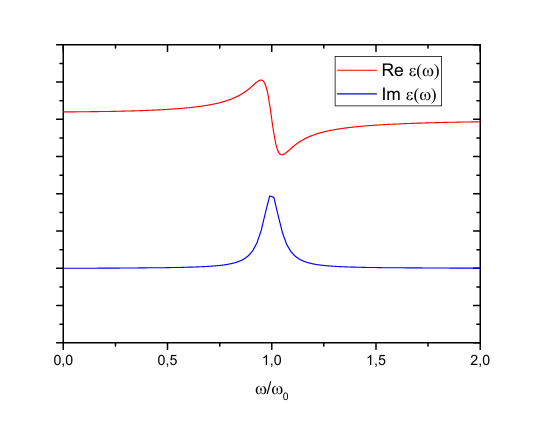
\includegraphics[width=0.4\textwidth]{Screenshot 2025-10-28 133819.png}

\columnbreak
    
\begin{equation}
    Re(\epsilon_r) = 1 + \frac{\omega^2_p(\omega_0^2 - \omega^2) }{(\omega_0^2 - \omega^2)^2 + \gamma^2\omega^2} 
\end{equation}

\begin{equation}
    Im(\epsilon_r) = \frac{\gamma \omega\omega_p^2}{(\omega_0^2 - \omega^2)^2 + \gamma^2\omega^2}
\end{equation}

\end{multicols}


Sorprendentemente, il modello può anche essere esteso per comprendere la conduttività. Se infatti poniamo $\omega_0 = 0 $ per alcuni elettroni, cioè poniamo a $0$ la forza di richiamo verso il nucleo, allora la costante dielettrica diventa singolare per $\omega = 0$: 

\begin{equation}
    \epsilon_r(\omega) = \epsilon_d + i\frac{\omega_p^2}{\omega(\gamma - i\omega)}
\end{equation}

Per capire la singolarità, consideriamo la quarta eq. di Maxwell
\begin{equation}
    \nabla \times H = J + \partial_t D
\end{equation}

Per un conduttore ohmico, si ha che $J = \sigma E$, mentre $D = \epsilon_0 \epsilon_d E$. L'eq. diventa allora 
\begin{equation}
    \nabla \times H = \left[\sigma + \epsilon_0 \epsilon_d\partial_t\right]E
\end{equation}

Assumendo un campo armonico, scriveremo 
\begin{equation}
    \nabla \times H = \left[\sigma - \epsilon_0\epsilon_d i\omega\right]E = -i\omega \epsilon_0 \left[\epsilon_d(\omega) + \frac{i\sigma}{\omega \epsilon_0}\right]E
\end{equation}

D'altra parte, se non avessimo inserito la legge di Ohm avremmo scritto
\begin{equation}
    \nabla \times H = -i\omega \epsilon_0 \epsilon_r(\omega)E
\end{equation}

Così che 
\begin{equation}
    \epsilon_r(\omega) = \epsilon_d + \frac{i\sigma}{\omega\epsilon_0} = \epsilon_d + i\frac{\omega_p^2}{\omega(\gamma - i\omega)}
\end{equation}

Che invertita ci dà una semplice espressione per la conduttività, 
\begin{equation}
    \sigma = \epsilon_0 \frac{\omega_p^2}{\gamma - i\omega}
\end{equation}

Tornando ai dielettrici, se vale $\omega >> \omega_0$, allora la costante dielettrica assume la semplice forma 
\begin{equation}
    \epsilon_r(\omega) = 1 - \frac{\omega_p^2}{\omega^2}
\end{equation}

Discutiamo un po' del numero d'onda: in questo limite è dato da 
\begin{equation}
    ck = \sqrt{\omega^2 - \omega_p^2}
\end{equation}

In certe situazioni, come un plasma di elettroni o nella ionosfera, il termine di damping $\gamma$ è nullo. In questi casi, si trova che la formula per il numero d'onda è valida anche per $\omega < \omega_0$, dove osserviamo che diventa un numero puramente immaginario. Questo risulta in una rapida decrescenza esponenziale dell'onda nel mezzo. 

\section{Plasmoni superficiali}

I plasmoni superficiali sono delle onde elettromagnetiche che si propagano nell'interfaccia fra un metallo ed un dielettrico. Sono confinate all'interfaccia, nel senso che decrescono esponenzialmente con coefficenti di assorbimento $\alpha_A, \alpha_M$ all'interno dei materiali ($A$ dielettrico, $M$ metallo). In formule, scriveremo che i campi elettrici sono dati da 

\begin{equation}
    E^{(A)} = (A, 0, B)e^{i(kx - \omega t)}e^{-\alpha_Az}
\end{equation}
\begin{equation}
    E^{(M)} = (C, 0, D)e^{i(kx - \omega t)}e^{\alpha_Mz}
\end{equation}

Se immaginiamo che la zona avente $z>0$ sia il materiale dielettrico, e la zona avente $z<0$ il metallo. \\

Le eq. di Maxwell per il campo elettrico sono in questo regime date da 

\begin{equation}
    \left(\nabla^2 + \frac{\epsilon_r\omega^2}{c^2} \right)E = 0 
\end{equation}

Possiamo calcolare allora il laplaciano nelle due zone, che darà 

\begin{align}
    \nabla^2 \vec{E} = \begin{cases}
        (-k^2 +\alpha_A^2)\vec{E}, \quad z > 0 \\ 
        (-k^2 +\alpha_M^2)\vec{E}, \quad z<0 
    \end{cases}
\end{align}

Da cui otteniamo le equazioni

\begin{align}
    &\alpha_A^2 = k^2 - \frac{\eps_A\omega^2}{c^2} \\
    &\alpha_M^2 = k^2 - \frac{\eps_M\omega^2}{c^2}
\end{align}
Inoltre è necessario imporre le condizioni al contorno. Come al solito, queste sono date da 

\begin{enumerate}
    \item conservazione di $E_{\parallel}$ \\
    La componente parallela è quella delle $x$. La condizione impone dunque semplicemente $A = C$. 
    \item conservazione di $D_{\perp}$\\
    La componente perpendicolare è quella in direzione $z$. Chiaramente, $D^{(A)} = \epsilon_0\epsilon_A E^{(A)}, \, D^{(M)} = \epsilon_0\epsilon_ME^{(M)}$, così che la condizione implica 
    \begin{equation}
        \epsilon_A B = \epsilon_M D
    \end{equation} 
\end{enumerate}


Notiamo inoltre che la prima equazione di Maxwell $\nabla \cdot E = 0$ nei due mezzi ci dicono che 
\begin{align}
    &iAk -B\alpha_A = 0 \\
    & iCk -D\alpha_M = 0 
\end{align}

usando le condizioni al contorno, posso sottrarre le equazioni ed ottenere

\begin{align}
    -B\alpha_M + D\alpha_A = 0 \implies -B\alpha_A + \frac{\eps_A}{\eps_M}\alpha_M B = 0 \implies \frac{\eps_A}{\alpha_A} = \frac{\eps_M}{\alpha_M}
\end{align}


Ora dobbiamo fare un po' di algebra per ottenere le relazioni di dispersione, \(k = k(\omega | \eps_A, \eps_M)\): fai il quadrato dell'ultima equazione, per ottenere

\begin{align}
    \frac{k^2 - \eps_A\frac{\omega^2}{c^2}}{\eps_A^2} = \frac{k^2 - \eps_M\frac{\omega^2}{c^2}}{\eps_M^2} 
\end{align}

Vogliamo ottenere una relazione per i \(k\), quindi spostiamoli a destra e raccogliamo: 

\begin{align}
    k^2\left(\frac{1}{\eps_A^2} - \frac{1}{\eps_M^2} \right) = \left(\frac{\omega}{c} \right)^2 \left(\frac{1}{\eps_A} - \frac{1}{\eps_M} \right)
\end{align}

Fai denominatore comune e semplifica: 

\begin{align}
    k^2 \left(\frac{\eps_M^2 - \eps_A^2}{\eps_A\eps_M} \right) = \left(\frac{\omega}{c} \right)^2(\eps_M -\eps_A) \implies k^2 = \left(\frac{\omega}{c} \right)^2\left(\frac{\eps_A\eps_M}{\eps_A + \eps_M} \right) 
\end{align}

Infine, abbiamo trovato che deve valere 

\begin{align}
    k(\omega | \eps_A, \eps_M) = \left(\frac{\omega}{c}\right)\sqrt{\frac{\eps_A\eps_M}{\eps_A + \eps_M}}
\end{align}

Questa \emph{non} è una relazione di dispersione lineare, perchè abbiamo visto nella sezione precedente come con il modello di lorentz sia possibile ottenere per un conduttore \(\eps_r(\omega)\). In particolare se vale \(\omega >> \omega_0\), allora potremo scrivere che la \(\chi(\omega)\) è in ottima approssimazione data da 

\begin{align}
    \chi(\omega) = -\frac{\omega_p^2}{\omega^2}
\end{align}

e la costante dielettrica 

\begin{align}
    \eps_M = 1 -  \frac{\omega_p^2}{\omega^2}
\end{align}

assumendo \(\eps_A\) reale e positiva, scriveremo allora che la relazione di dispersione completa per un plasmone superficiale è data da 

\begin{align}
    k(\omega) = \left(\frac{\omega}{c}\right)\sqrt{\frac{\eps_A\left(1 - \frac{\omega_p^2}{\omega^2}\right)}{\eps_A + 1 - \frac{\omega_p^2}{\omega^2}}} = \left(\frac{\omega}{c} \right)\sqrt{\frac{\eps_A(\omega^2 - \omega_p^2)}{\omega^2(\eps_A + 1)-\omega_p^2}}
\end{align}

Un grafico della relazione di dispersione è il seguente (parametri \(c=10, \omega_p = 1, \eps_A = 2\)): 

\begin{center}
\begin{tikzpicture}[scale=0.7]
        \begin{axis}[
        ymin =0, ymax= 0.5, 
        xmin=0, xmax=5, 
        xlabel = {$\omega$},
        ylabel = {$k(\omega)$},
        grid = both,                % griglia
        grid style = {dashed, gray!30},
        axis lines = left,          % assi più puliti
        thick, % linee più spesse
    ]


    \addplot[color=doc, samples=200, domain = 0: 3^(-1/2)]{(x/10)*((2*(x^2-1))/(3*x^2-1))^(1/2)};

    \addplot[color=doc, samples=200, domain = 1: 5]{(x/10)*((2*(x^2-1))/(3*x^2-1))^(1/2)};

    \addplot[color=black, samples=10, dashed]{(2)^(1/2)*x/10};

    \addplot[color=purple, samples=10, dashed]{(2/3)^(1/2)*x/10};

    \node at (axis cs:4, 0.25)[color = purple] {$ \sqrt{\frac{\eps_A}{\eps_A +1}}$};

    \node at (axis cs:1, 0.2) [color = black]{$ \sqrt{\eps_A}$};

    \draw[->, thick, black](axis cs: 0, 0.9) --(axis cs: 2, 0.9); 


    \end{axis}
    \end{tikzpicture}
\end{center}

Vediamo che nei limiti per \(\omega \rightarrow 0\) e \(\omega \rightarrow \infty\) la relazione diventa lineare. In effetti, vale chiaramente che 

\begin{align}
    &k \simeq \left(\frac{\omega}{c} \right)\sqrt{\frac{-\eps_A \omega_o^2}{-\omega_p^2}} = \frac{\sqrt{\eps_A}\omega }{c} \\
    &k \simeq \left(\frac{\omega}{c}\right)\sqrt{\frac{\omega^2\eps_A}{\omega^2(\eps_A+1)}} = \sqrt{\frac{\eps_A}{\eps_A + 1}}\left(\frac{\omega}{c} \right)
\end{align}

Come è possibile osservare anche in figura. Inoltre, il denominatore tende a \(0\) per \(\omega \rightarrow \frac{\omega_p}{\sqrt{\eps_A +1}}\), che risulta chiaramente in un asindoto verticale. Per \(\omega \in \left(\frac{\omega_p}{\sqrt{\eps_A +1}}, \omega_p\right)\), la radice è negativa e la funzione non è ben definita. Questo vuol dire che non esistono modi con queste frequenze. Le due regioni invece dove i modi esistono sono più interessanti: 

\begin{enumerate}
    \item \(\omega > \omega_p\): \\
    In questa regione, vale \(k < \frac{\omega}{c}\sqrt{\frac{\eps_A}{\eps_A +1}} < \frac{\omega}{c}\sqrt{\eps_A}\). Questi modi sono detti \emph{radiativi}, oppure \emph{modi di Brewster}. Questi non sono confinati alla interfaccia ma propagano, perchè valendo 
    
    \begin{align}
        \alpha_A^2 = k^2 - \left(\frac{\omega}{c} \right)^2\eps_A < 0
    \end{align}

    Il coefficiente \(\alpha_A\) è puramente immaginario. Si può vedere che vale lo stesso anche per \(\alpha_M\): in effetti, vale 

    \begin{align}
        \alpha^2_M = k^2  - \eps_M \frac{\omega^2}{c^2} 
    \end{align}

    sostituendo la relazione \(k = \omega/c \sqrt{\frac{\eps_A\eps_M}{\eps_A + \eps_M}}\), otteniamo che 

    \begin{align}
        \alpha_M^2 &= \left(\frac{\omega}{c} \right)^2\left(\frac{\eps_A\eps_M}{\eps_A + \eps_M} -\eps_M\right) \\
        &= \eps_M \left( \frac{\omega}{c}\right)^2 \left(\frac{\eps_A - \eps_A - \eps_M}{\eps_A + \eps_M} \right) = -\frac{\eps_M^2 }{\eps_A + \eps_M}\left(\frac{\omega}{c} \right)^2 < 0
    \end{align}

    dunque sono onde che si propagano in entrambi i materiali. Sono detti di Brewster perchè è possibile ottenere la condizione di Brewster per l'onda incidente, se vale 

    \begin{align}
        \tan\theta_B = \sqrt{\eps_A/\eps_M}
    \end{align}

    \item \(\omega < \frac{\omega_p}{\sqrt{\eps_A + 1}}\): \\
    Questi sono i \emph{modi di Fano}. Si tratta di modi confinati, perchè i coefficienti \(\alpha_A, \alpha_M\) sono reali e positivi. Questi sono quindi i plasmoni superficiali che stavamo cercando. 

\end{enumerate}

In particolare, i modi di fano non possono essere eccitati da onde provenienti dal mezzo dielettrico (\(A\)). Questo perchè l'onda indicidente ha \(k = \omega/c \sqrt{\eps_A}\sin\theta < \omega/c \sqrt{\eps_A}\), quindi non è abbastanza alta per "matchare" la curva di dispersione. \\
Esiste però un modo per eccitare lo stesso le onde, usando la tecnica della riflessione totale. Si inserisce in pratica un'altro strato di dielettrico \(P\), con \(n > \sqrt{\eps_A}\). Un'onda che arriva dal mezzo p ha vettore d'onda \(k = \omega/c n_p \sin\theta\), che può essere abbastanza grande per arrivare alla curva del plasmone, e penetra nel dielettrico con uno smorzamento esponenziale. Tipicamente, si riesce ad eccitare plasmoni in questo modo, usando ad esempio un prisma ed un sottile film metallico, e come altro dielettrico il vuoto.  

\section{Guide d'onda}

    Rivolgiamo ora la nostra attenzione verso la propagazione di onde elettromagnetiche all'interno di guide metalliche. Questo è interessante perchè mostra come, date appropriate condizioni al contorno, l'eq. agli autovalori di Helmotz ha uno spettro discreto, esattamente come succede in meccanica quantistica quando ho uno stato legato. \\

    Consideriamo dunque una guida con sezione costante, con asse parallelo all'asse $z$. Se consideriamo onde elettromagnetiche, i campi soddisfano l'equazione di Helmotz: 

    \begin{equation}
        \left(\nabla^2 + \omega^2 \epsilon\mu \right) \left\{\begin{matrix}
            E \\ B 
        \end{matrix} \right\}
         = 0
    \end{equation}

    Guidati dalla simmetria del problema, vorremmo cercare delle soluzioni che propagano lungo la direzione $z$, con un costante profilo d'onda lungo $x,y$. In formule, cerchiamo delle soluzioni del tipo 
    \begin{align}
        E = E(x, y)e^{i(kz - \omega t)} \\ B = B(x, y)e^{i(kz - \omega t)} 
    \end{align}


    Osserviamo quindi che nel nostro caso, l'operatore laplaciano agisce sui campi secondo 
    \begin{equation}
        \nabla^2 = \partial_x^2 + \partial_y^2 + \partial_z^2 = \nabla_T^2 - k^2
    \end{equation}

    Dove col simbolo $\nabla^2_T$ abbiamo indicato il laplaciano nelle direzioni trasverse. Sotto queste ipotesi, l'eq. di Helmotz diventa 

    \begin{equation}
        \left(\nabla_T^2 + \gamma^2 \right) \left\{\begin{matrix}
            E \\ B 
        \end{matrix} \right\}
         = 0
    \end{equation}

    Dove abbiamo identificato $\gamma^2 = \omega^2\epsilon\mu - k^2$. \\

    Consideriamo ora le componenti trasverse, partendo dalle eq. di Maxwell del primo ordine: abbiamo 

    \begin{align}
        &\nabla \times B = \epsilon\mu \partial_t  E \xrightarrow{componente \, x} -i\omega \epsilon\mu E_x = \partial_y B_z -ikB_y  \\
        &\nabla \times E = -\partial_tB \xrightarrow{componente \, y} i\omega B_y= ikE_x  -\partial_xE_z \\
    \end{align}

    Per combinare le due espressioni, moltiplico per $i\omega$ la prima, e usando la seonda sostituisco $i\omega B_y$, per ottenere: 

    \begin{align}
        &\omega^2 \epsilon\mu E_x= i\omega \partial_y B_z +ik(\partial_xE_z -ikE_x) \\ &(\omega^2 \epsilon\mu- k^2)E_x = i (\omega \partial_yB_z + k\partial_xE_z)
    \end{align}

    Riconoscendo l'espressione per $\gamma$, scriviamo dunque 
    \begin{equation}
        E_x = \frac{i}{\gamma^2}(\omega \partial_yB_z + k\partial_xE_z)
    \end{equation}
    Similmente, si ottiene anche 
    \begin{equation}
        E_y = \frac{-i}{\gamma^2}(\omega \partial_yB_z - k\partial_xE_z)
    \end{equation}
    E per il campo magnetico 
    \begin{equation}
        B_x = \frac{-i}{\gamma^2}(\omega \epsilon\mu\partial_yE_z - k\partial_xB_z)
    \end{equation}
    \begin{equation}
        B_y = \frac{i}{\gamma^2}(k \partial_yB_z + \omega\epsilon\mu\partial_yE_z)
    \end{equation}
    
    In particolare, abbiamo imparato che dati $E_z, B_z$ i campi trasversi sono immediati da determinare. Vi sono due possibili modi: 
    \begin{enumerate}
        \item TM \\ In questo si ha $B_z =0, \, E_z \neq 0$. \\
        Le condizioni al contorno rilevanti sono date dalla conservazione di $E_{\parallel}$. In particolare, la direzione parallela alla guida è $z$, così che deve valere sul bordo della guida 
        \begin{equation}
            E_z |_{S} = 0 
        \end{equation}
        \item TE \\ $B_z \neq 0, \, E_z = 0 $. \\
        La condizione da imporre è ora che si conservi $B_{\perp}$. Questo ci dice che deve valere $B_x|_S = B_y|_S = 0$. D'altra parte, combinate con le relazioni precedenti per le componenti $B_x, B_y$, queste condizioni impongono delle condizioni sulla componente $z$: 
        \begin{equation}
            \partial_xB_z|_S = 0, \quad \partial_yB_z|_S = 0
        \end{equation}
    \end{enumerate}

    Uno potrebbe chiedersi anche dei modi TEM, dove $E_z = B_z = 0$. In questi casi, si ottiene che tutti i campi sono nulli, date le espressioni ricavate prima. \\

    Per riassumere le eq. da risolvere nelle situazioni rilevanti sono: 

    \begin{tcolorbox}[colback=doc!15, colframe=black, boxrule=1pt]
    \begin{align}
        &(\nabla^2 + \gamma^2)E_z = 0, \quad E|_S = 0 \quad (\text{TM})\\ &(\nabla^2 + \gamma^2)B_z = 0, \quad \partial_nB|_S = 0 \quad (\text{TE}) 
    \end{align}
    \end{tcolorbox}

    Già intuitivamente, si può comprendere la natura delle soluzioni di queste equazioni. Si tratta di equazioni oscillanti, che si annullano (o si annullano le loro derivate) a degli estremi fissati. In questo senso, sono molto simili alle autofunzioni della buca di potenziale infinita. \\

    La cosa più interessante di questi modi sono le leggi di dispersione. Poichè lo spettro è discreto, vi sarà un set discreto di $\gamma_n$, che soddisfi: 

    \begin{equation}
        \gamma_n^2 = \omega^2\epsilon\mu - k^2
    \end{equation}
    Le condizioni al contorno implicano che $k$ sia reale (se l'andamento dei campi è esponenziale non possono annullarsi al bordo). D'altra parte, risolvendo per $k$ troviamo che 
 
    \begin{equation}
        k_n = \frac{n}{c}\sqrt{\omega^2 - \omega_n^2}, \quad \omega_n := \frac{c}{n}\gamma_n
    \end{equation}

    \begin{center}
        \begin{tikzpicture}[scale=0.7]
        \begin{axis}[
        ymin =0, ymax= 0.6, 
        xmin=0, xmax=5, 
        xlabel = {$\omega$},
        ylabel = {$k(\omega)$},
        grid = both,                % griglia
        grid style = {dashed, gray!30},
        axis lines = left,          % assi più puliti
        thick, % linee più spesse
    ]


    \addplot[color=doc, samples=200, domain = 1:5]{(1/10)*(x^2 - 1)^(1/2)};

    \addplot[color=purple, samples=200, domain = 2:5]{(1/10)*(x^2 - 4)^(1/2)};


    \node at (axis cs:2, 0.25)[color = doc] {$ \omega_n = 1$};
    \node at (axis cs:4, 0.25)[color = purple] {$ \omega_n = 2$};


        \end{axis}
        \end{tikzpicture}
    \end{center}

    In grafico sono rappresentati due possibili modi. 

    Esistono dunque diversi modi $k_n(\omega)$, ma tutti si accendono dopo la frequenza di \emph{cutoff} $\omega_n$: prima non vi sono soluzioni che rispettino le condizioni al contorno \footnote{Sarebbe meglio specificare, che non è possibile avere modi con pulsazioni \emph{reali} con frequenze inferiori ad \(\omega_n\). In effetti, dalla legge di dispersione si ottiene che per \(\omega < \omega_p\), \(k\) diventa puramente immaginario, e questo porta ad un campo trasverso che decresce esponenzialmente con la distanza.}. Con i soliti calcoli si trovano anche poi velocità di fase e di gruppo: 

    \begin{align}
        &v_{ph} = \frac{c}{n}\sqrt{1 + \frac{\gamma_n^2}{k^2}} \\ &v_{gr} = \frac{c}{n}\frac{1}{\sqrt{1 + \frac{\gamma_n^2}{k^2}}}
    \end{align}

    \ex{}{
        Vediamo come si trasmettono delle onde all'interno di una guida \emph{rettangolare}, di lati $a, b$. Consideriamo il caso TM: l'equazione da risolvere è data da 
        \begin{equation}
            (\partial_x^2 + \partial_y^2 + \gamma^2)E_z(x, y) = 0 
        \end{equation}
        Per risolverla, suppongo che valga $E_z(x, y) = \phi(x)\psi(y)$. Avendo fatto questo ansatz, l'eq. si scompone in 
        \[\begin{cases}
            \phi'' = -\gamma_x^2\phi \\ \psi'' = -\gamma_y^2 \psi 
        \end{cases}\]

        Le soluzioni di queste sono chiaramente date da 
        \begin{align}
            &\phi(x) = A\sin(\gamma_x x) + B\cos(\gamma_x x) \\ &\psi(y) = A\sin(\gamma_y y) + B\cos(\gamma_y y)
        \end{align}

        Ora è tempo di imporre le condizioni al contorno: 
        \begin{equation}
            \phi(0) = \psi(0) = 0 \rightarrow A = 0 
        \end{equation}
        \begin{equation}
            \phi(a) = \psi(b) = 0 \rightarrow \gamma_x = \frac{\pi}{a}n, \, \gamma_y = \frac{\pi}{b}m
        \end{equation}

        Abbiamo dunque trovato 
        \begin{equation}
            \gamma_{m, n} = \pi \sqrt{\frac{m^2}{a^2} + \frac{n^2}{b^2}}
        \end{equation}

        Questo mostra che, supponendo $a<b$, che non vi sono soluzioni aventi una frequenza minore di 
        \begin{equation}
            \omega_{1, 0} = \frac{c\pi}{a}
        \end{equation}
        Possiamo anche scrivere la soluzione esplicita dell'equazione, data da 
        \begin{equation}
            E_z(x, y) = E_0\sin\left(\frac{\pi m x}{a}\right)\sin\left(\frac{\pi n x}{b}\right)
        \end{equation}
    }

    Se invece la guida d'onda non si estende all'infinito, ma ha una lunghezza $L$? In questo caso, devo imporre le condizioni al contorno anche alla componente $z$. Il risultato che si ottiene è che la frequenza è completamente discreta: 


    Se si tratta di un onda TE scriveremo
    \begin{equation}
        B_z = (A\cos(kz)+B\sin(kz))\phi(x)\psi(y)
    \end{equation}
    e dobbiamo imporre le condizioni al contorno $B_z|_S = 0$. Questo richiede che valga $A=0, kL = \pi j, j \in \mathbb{Z}$. La pulsazione è dunque completamente discretizzata, 
    \begin{equation}
        \omega = c\pi\sqrt{\frac{ j^2}{L^2} + \frac{m^2}{a^2}+ \frac{n^2}{b^2}}
    \end{equation}


    \section{Materiali con indici di rifrazione negativo}

    Veselago in un articolo del '68, indagò l'apparente assimetria, dovuta al fatto che si osservano materiali solo con \(\eps, \mu >0\). Concluse alla fine della sua ricerca, che materiali con permettività elettrica e permeabilità magnetica inferiori a zero dovrebbero in realtà esistere. Nella maggior parte dei casi, i due termini appaiono in prodotto fra di loro, così che il loro segno individuale, se è concorde, non gioca un effetto. D'altra parte, nelle equazioni di Maxwell i due termini appaiono anche non accoppiati, ad esempio nelle formule dei rotori: 

    \begin{align}
        \vec{\nabla}\times \vec{E} &= -\frac{\partial\vec{B}}{\partial t} \\
        \vec{\nabla} \times \vec{H} &= \frac{\partial \vec{D}}{\partial t}
    \end{align}


    Nel caso di un materiale lineare, e di campi armonici, infatti, queste equazioni diventano: 

    \begin{align}
        \vec{\nabla}\times \vec{E} &=  i\omega \mu \vec{H} \\
        \vec{\nabla} \times \vec{H} &= -i\omega \eps \vec{E}
    \end{align}

    Se poi ho un'onda piana, posso sostituire \(\vec{\nabla} \rightarrow i\vec{k}\), così da ottenere 

    \begin{align}
        \vec{k}\times \vec{E} &= \omega \mu \vec{H} \\
        \vec{k}\times \vec{H} &= -\omega \eps \vec{E}
    \end{align}


    Ora, nel caso in cui le costanti sono positive, allora la terna \(\vec{k}, \vec{E}, \vec{H}\) è una terna destrorsa, ma se sono negativi no! D'altra parte, il vettore di Poynting è sempre dato da 

    \begin{align}
        \vec{S} = \vec{E} \times \vec{H}
    \end{align}

    quindi in particolare forma sempre una terna destrorsa con gli altri due, e come al solito indica la propagazione dell'energia, perchè è la quantità che entra nell'equazione dellla conservazione dell'energia. D'altra parte, se entrambe le costanti sono negative, si trova allora che i vettori \(\vec{k}, \vec{S}\) sono antiparalleli! Questo vuol dire che l'onda si propaga nel senso inverso dell'energia, all'interno di questi materiali. Poichè tipicamente si scrive che 

    \begin{align}
        \vec{k} = \frac{n}{c}\hat{n}
    \end{align}

    questi materiali sono tipicamente detti ad \emph{indice di rifrazione negativo}. Questi materiali hanno molte altre interessanti proprietà, ad esempio rifraggono la luce attraverso un angolo \emph{negativo}, cioè opposto alla direzione tipicamente osservata. Queste previsioni teoriche sono state confermate sia da simulazioni che da esperimenti, a frequenza delle onde molto elevata (\(\approx 12\) GHz).  

















    \chapter{Radiazione di cariche localizzate}

    Fino ad ora abbiamo considerato campi armonici, senza chiederci come questi vengano generati. In questa sezione vogliamo indagare come cariche e correnti oscillanti generano campi oscillanti. 

    Per prima cosa dunque, supporremo di avere delle distribuzioni di carica $\rho$ e delle densità di corrente $J$, che soddisfino

    \[\begin{cases}
        \rho(x, t) = \rho(x)e^{-i\omega t} \\ J(x, t) = J(x)e^{-i\omega t}
    \end{cases}\]

    A partire da queste, vorrei determinare la forma dei campi $E, B$. La strategia che seguiremo è la seguente: 
    \begin{enumerate}
        \item determino $A$ 
        \item determino $B$ \\
        Questo è semplice una volta noto $A$, perchè mi basta prendere $\nabla \times A$
        \item determino $E$ \\
        Una volta noto $B$, posso usare la legge di Ampere-Maxwell 
        \begin{equation}
            \nabla \times B = c^{-2}\partial_tE + \mu_oJ
        \end{equation}
        Poichè vorremo determinare i campi lontano dalle cariche, possiamo prendere $J=0$ nell'equazione precedente, così che anche il calcolo di $E$ sia in linea di principio banale. 
    \end{enumerate}

    Cominciamo dunque col calcolare il potenziale vettore. Sappiamo che questo, nel gauge di Lorentz, obbedisce all'equazione delle onde con termine di sorgente: 

    \begin{equation}
        \square A = -\mu_o J
    \end{equation}
    Di cui abbiamo già studiato la soluzione: 
    \begin{equation}
        A(x, t) = \frac{\mu_0}{4\pi}\int d^3x' \frac{J(x', t - \frac{|x'-x|}{c^2})}{|x'-x|}
    \end{equation}

    sostituendo l'espressione di $J$, 
    \begin{equation}
        A(x, t) = \frac{\mu_0}{4\pi}\int d^3x' \frac{J(x')}{|x'-x|}e^{-i\omega t + ik|x'-x|} = \frac{\mu_0e^{-i\omega t}}{4\pi} \underbrace{\int d^3x'\frac{J(x')}{|x'-x|}e^{ik|x'-x|}}_{:= A(x)}
    \end{equation}

    Osserviamo dunque già che la dipendenza da $t$ è la stessa fra $J, A$. In particolare, entrambi oscillano alla medesima frequenza. Invece, la forma di $A(x)$ dipende da come è fatto $J(x)$. In moltissime situazioni, il calcolo di $A(x)$ è particolarmente laborioso. Vogliamo fare dunque delle ipotesi che permettano alcune approssimazioni. \\

    Supporremo dunque che le cariche siano \emph{localizzate}, ovvero contenute in una regione di dimensione caratteristica $d$, t.c. $d << r$, con $r$ la distanza fra il punto dove vogliamo determinare il campo, e l'origine del mio sistema di riferimento. Scriveremo sempre che $\hat{n} = \frac{x'-x}{r}$, così che in questa approssimazione si avrà 
    \begin{equation}
        |x'-x| \simeq r - \hat{n}\cdot x'
    \end{equation}
    Infatti, vale 
    \begin{align}
        |x'-x| &= \sqrt{(x'-x)^2 + (y'-y^2)+(z'-z)^2} \\ &\simeq \sqrt{r^2 - 2(xx' + yy' + zz')} \simeq  r - \hat{n}\cdot x'
    \end{align}

    La lunghezza d'onda è definita a partire dal vettore d'onda come
    \begin{equation}
        \lambda = \frac{2\pi}{k}
    \end{equation}

    Siamo interessanti a due situazioni limite, in particolare: 
    \begin{enumerate}
        \item $d << \lambda << r$ \\
        Detto limite di \emph{far field}. 
        \item $d << r << \lambda$ \\
        detto limite di \emph{near field}. 
    \end{enumerate}

    Ora, usando l'ipotesi $d << r$, posso già scrivere 
    \begin{equation}
        A(x) = \frac{\mu_0}{4\pi}\frac{e^{ikr}}{r}\int d^3x' J(x')e^{-ik \hat{n}\cdot x'}\left(1 + \frac{\hat{n}\cdot x'}{r}+ ..\right)
    \end{equation}

    Dove abbiamo semplicemente sostituito $|x'-x| = r - \hat{n}\cdot x'$. Vediamo come l'espressione si semplifica ulteriormente nei due limiti: 

    \begin{enumerate}
        \item near field \\

        La condizione è $d << r << \lambda$. Moltiplicando tutto per $k$, ottengo 
        $kd << kr << 2\pi$. In questa regione dunque posso semplicemente, prendere il limite per $kr \rightarrow0$, così che varrà 
        \begin{equation}
            A(x) = \frac{\mu_0}{4\pi}\frac{1}{r}\int d^3x' J(x')\left(1 + \frac{\hat{n}\cdot x'}{r}+ .. \right)
        \end{equation}
        In particolare, osserviamo che 
        \begin{equation}
            A \approx \frac{1}{r} \rightarrow B = \nabla \times A \approx \frac{1}{r^2} \rightarrow E \propto \nabla \times B \approx \frac{1}{r^3}
        \end{equation}

        i campi risultanti, dunque, decrescono rapidamente con la distanza, e non trasportano energia fino all'infinito: in particolare, non sono i campi radiativi che cercavamo. 

        \item far field \\
        In questa regione, sempre moltiplicando per $k$, otteniamo che 
        \begin{equation}
            k\cdot x' << kr
        \end{equation}
        Possiamo dunque espandere in serie di Taylor l'esponenziale dentro l'integrale: 
        \begin{equation}
            e^{-ik\hat{n}\cdot x'} = \sum_{n=0}^{+\infty}\frac{(-ik)^n}{n!}(\hat{n}\cdot x')^n
        \end{equation}
        Così che scriveremo
        \begin{equation}
            A(x) = \frac{\mu_0}{4\pi}\frac{e^{ikr}}{r}\sum_{n=0}^{+\infty}\frac{(-ik)^n}{n!}\int d^3x' J(x')(\hat{n}\cdot x')^n\left(1 + \frac{\hat{n}\cdot x'}{r} + ..\right) 
        \end{equation}

        Questa scrittura del potenziale è detta \emph{espansione in multipolo}. \\

        \nt{Questa scrittura è utile nell'approssimazione far-field, perchè nota che valendo 
            \begin{align}
                d << \lambda
            \end{align}

        Moltiplicando per \(k\) si ottiene che 

        \begin{align}
            kd << k\lambda \approx 1
        \end{align}

        A questo punto è chiaro che la grandezza del termine n-esimo, data da 
        \begin{align}
            \frac{1}{n!}(k \vec{x}' \cdot \hat{n})^n
        \end{align}

        decresce rapidamente con \(n\), perchè \(|\vec{x'}|\) è dell'ordine di \(d\). 
        }
        

        \end{enumerate}

        \section{Termine di dipolo elettrico}
        
            Se nell'espressione far field per $A$ ci fermiamo al termine $n=0$, detto termine di \emph{dipolo elettrico}, l' espressione diventa
            \begin{equation}
                A_0(x) = \frac{\mu_0}{4\pi}\frac{e^{ikr}}{r}\int d^3x' J(x')
            \end{equation}

            Poichè la corrente è nulla all'infinito, potremmo integrare per parti ed ottenere 
            \begin{equation}
                A_0(x) = -\frac{\mu_0}{4\pi}\frac{e^{ikr}}{r}\int d^3x' x (\nabla \cdot J)
            \end{equation}
            Usando l'eq. di continuità, scriveremo 
            \begin{equation}
                \nabla \cdot J = -\partial_t\rho = i\omega \rho
            \end{equation}
            Così che scriveremo 
            \begin{equation}
                A_0(x) = \frac{-i\omega \mu_0}{4\pi}\frac{e^{ikr}}{r}\underbrace{\int d^3x' x \rho(x)}_{:=p}
            \end{equation}
            Dove abbiamo definito il vettore dipolo elettrico. Si scrive dunque infine 
            \begin{equation}
                A_0(x) = \frac{-i\mu_0}{4\pi}(ck)\frac{e^{ikr}}{r}p 
            \end{equation}
            Come sono fatti i campi $E, B$? Bisogna fare un po' di derivate: 
            \begin{align}
                B &= \nabla \times A_0 = \frac{-i\mu_0}{4\pi}(ck) \nabla \times \left( \frac{e^{ikr}}{r}p\right) \\
                &= \frac{-i\mu_0}{4\pi}(ck) \left(\nabla\left(\frac{e^{ikr}}{r}\right)\times p + \frac{e^{ikr}}{r}(\nabla \times p) \right)
            \end{align}

            Ora calcoliamo 
            \begin{equation}
                \nabla\left(\frac{e^{ikr}}{r} \right) = \frac{d}{dr}\left(\frac{e^{ikr}}{r} \right)\hat{n} = \left(\frac{ik}{r} - \frac{1}{r^2} \right)e^{ikr}\hat{n}
            \end{equation}
            Si ottiene così 
            \begin{equation}
                B = ck^2 \frac{\mu_0}{4\pi}\left(1 - \frac{1}{ikr} \right)\frac{e^{ikr}}{r}(\hat{n}\times p )
            \end{equation}

            Similmente si può calcolare l'espressione per $E$, data da 
            \begin{align}
                E &= \frac{ic}{k}(\nabla \times B) \\
                &= \frac{1}{4\pi\epsilon_0}\left\{\frac{k^2}{r}(\hat {n}\times p) \times \hat{n} + (3(\hat{n}\cdot p)\hat{n}-p)\left(\frac{1}{r^3}- \frac{ik}{r^2}\right)\right\}e^{ikr} \\
                &\simeq c (B \times \hat{n})
            \end{align}

            Dove l'ultima è una approssimazione valida per \(r \rightarrow \infty\). In generale, il campo elettrico ha componenti sia parallele, sia ortogonali ad \(\hat{n}\) (le prime, in ogni caso, è possibile mostrare che descrescano con \(r^{-3}\)). 


            Dati i campi, è interessante calcolare il vettore di Poynting, dato da 
            \begin{equation}
                S = \frac{1}{2\mu_0}\text{Re}(E\times B^{*}) \simeq \frac{c}{2\mu_0}\text{Re}((\hat{n}\times B)\times B) = \frac{c}{2\mu_0}|B|^2\hat{n}
            \end{equation}
            Sostituendo l'espressione per $B$, troviamo 
            \begin{equation}
                S = \frac{c}{2\mu_o}\frac{k^4}{16\pi^2\epsilon_0^2 c^2}\left( \frac{1}{r^2}\right)|\hat{n}\times p|^2 = \frac{ck^4}{32\pi^2\epsilon_0}\left( \frac{1}{r^2}\right)|\hat{n}\times p|^2 = \frac{ck^4}{32\pi^2\epsilon_0}\left( \frac{1}{r^2}\right)|p|^2 \sin^2 \theta 
            \end{equation}
            Dove abbiamo indicato con \(\theta\) l'angolo compreso fra \(\vec{p}, \hat{n}\). \\
            Il fatto che $S \propto r^{-2}$ è importante, perchè la potenza totale irraggiata è data da 
            \begin{equation}
                P = \int (S\cdot \hat{n})r^2 d\Omega
            \end{equation}
            Così che la potenza irraddiata per angolo solido $\frac{dP}{d\Omega}$ sia indipendete dal raggio $r$. 

            In particolare, troviamo che 
            \begin{equation}
                \frac{dP}{d\Omega} = (S\cdot \hat{n})r^2 = \frac{ck^4}{32\pi^2\epsilon_0}p^2\sin^2\theta
            \end{equation}

            La potenza totale si ottiene poi integrando sull'angolo solido, 
            \begin{align}
                P &= \frac{ck^4}{32\pi^2\epsilon_0}p^2\underbrace{\int_0^{2\pi} d\varphi \int_0^{\pi} d\theta \sin^2\theta}_{= (8/3)\pi} \\
                &= \frac{ck^4}{12\pi \epsilon_0}p^2
            \end{align}

            I termini successivi (per $n\geq 1$) sono poco interessanti e molto calcolosi. In particolare, il termine $n=1$ è detto di dipolo magnetico e quadrupolo elettrico. 

    \section{Scattering a grandi lunghezza d'onda}

    Ci occupiamo ora di affrontare il problema di come un campo indidente viene scatterato da un mezzo lineare, di dimesioni $a$ molto più piccole della lunghezza d'onda $\lambda$. Lo scattering è dovuto al fatto che il campo incidente induce dei dipoli magnetici ed elettrici nel mezzo, che poi iraddiano in direzioni anche diverse da quella incidente. Il fatto di considerare grande lunghezze d'onda ci permette di fermarci nell'espansione in multipoli ai termini di dipolo elettrico e magnetico. \\

    Siccome il mezzo è lineare, varrà allora 
    \begin{equation}
        p = \epsilon_0 \alpha E_{inc}
    \end{equation}

    Inoltre se ha forma sferica, 
    \begin{equation}
        \alpha = 4\pi \left(\frac{n^2-1}{n^2+1} \right)a^3
    \end{equation}

    Abbiamo imparato che un campo elettrico generato da un dipolo elettrico è dato da 
    \begin{equation}
        E = \frac{k^2}{4\pi\epsilon_0}[(\hat{n}\times p)\times \hat{n}]\left(\frac{e^{ikr}}{r} \right)
    \end{equation}

    Definiamo allora la sezione d'urto differenziale nel seguente modo: (potenza per angolo solido della radiazione scatterata, fratto l'intensitò dell'onda incidente)
    \begin{equation}
        \frac{d\sigma}{d\Omega} = \frac{\frac{dp}{d\Omega}}{I_{inc}} = \frac{r^2[\hat{e}\cdot E_{sc}]^2}{[\hat{e}_0 \cdot E_{inc}]^2}
    \end{equation}
    Così da trovare, sostituendo l'espressione per 
    \begin{tcolorbox}[colback=doc!15, colframe=black, boxrule=1pt]
    \begin{equation}
        \frac{d\sigma}{d\Omega} = \frac{k^4}{16\pi^2\epsilon_0^2}\frac{|\hat{e}\cdot p|^2}{E_o^2} = \frac{k^4\alpha^2}{16\pi^2}|\hat{e}\cdot \hat{e_0}|^2
    \end{equation}
    \end{tcolorbox}

    Osserviamo in particolare: 
    \begin{enumerate}
        \item La dipendenza $\propto k^4 \propto \lambda^{-4}$ \\
        Questa è nota come legge di Rayleigh ed è la ragione per cui il cielo appare azzurro: le lunghezze d'onda più alte sono scatterate di più dall'atmosfera.
        \item Il termine $|\hat{e}\cdot \hat{e}_0|^2$ \\ 
        Questo introduce una dipendenza angolare, perchè possiamo prendere
        \begin{equation}
            \hat{e}_0 = \sin\phi \hat{e}_{0, \parallel} + \cos\phi \hat{e}_{0, \perp} 
        \end{equation}
        Così che valga 
        \begin{equation}
            |\hat{e}\cdot \hat{e}_0|^2 = \frac{1}{2}(1+\cos^2\theta)
        \end{equation}
        Dove $\theta$ è l'angolo compreso fra i due versori. \\
        Potremmo in particolare scomporre la sezione d'urto in una dipendente dall'angolo e non dipendente: 
        \begin{equation}
            \left(\frac{d\sigma}{d\Omega}\right)_{\parallel} = \frac{k^4\alpha^2}{16\pi^2}\left(\frac{1}{2}\cos^2\theta \right), \quad \left(\frac{d\sigma}{d\Omega}\right)_{\perp} = \frac{k^4\alpha^2}{32\pi^2}
        \end{equation}

    \end{enumerate}

\newpage

\chapter{Relatività ristretta}

\section{Una introduzione "storica"}

Quando Maxwell pubblicò il suo trattato, nel 1882, la meccanica era al suo massimo storico. Questo non è un caso: dopo aver spiegato la termodinamica attraverso la meccanica statistica, insieme a Boltzmann, il vero obbiettivo del lavoro di Maxwell era di unificare anche l'elettromagnetismo con la meccanica. Non c'è da stupirsi, allora, che quando Maxwell ricavo l'equazione delle onde per i campi $E, B$

\begin{equation}
    \left(\nabla^2 + \frac{1}{c^2}\frac{\partial^2}{\partial t^2} \right)E = 0 
\end{equation}

e si accorse che questa non era invariante sotto il gruppo di trasformazioni di Galileo \footnote{Per vederlo, basta effettuare le derivate nelle nuove componenti: da una parte vale $\partial^2_t = \partial^2_{t'}$, dall'altra $\partial_{x'} = (\partial_{x'} x)\partial_x + (\partial_{x'}t)\partial_t = \partial_x - v\partial_t$}
\[\begin{cases}
    x' = x-vt \\ t' = t
\end{cases}\]

ma piuttosto sotto il gruppo di trasformazioni di Lorentz: 
\[\begin{cases}
    x' = \gamma (x - vt) \\ y' = y \\ z' = z \\ t' = \gamma \left(t - \frac{v}{c^2}x\right)
\end{cases}\]

lui semplicemente suppose che queste dovevano valere in un sistema di riferimento speciale, solidale al mezzo in cui le onde si propagavano, l'\emph{etere}. \\

Negli anni seguenti, (dal 1887 fino a circa 50 anni dopo), furono eseguiti diversi esprimenti per misurare il moto della terra rispetto all'etere. Il più famoso di questi fu l'esperimento di Mikelson-Morley. Di fatto, nessuno di questi esprimenti rivelò il moto della terra rispetto all'etere. Questo fece interessare diversi teorici alla materia. \\

Nel 1905, Einstein pubblico un'articolo "sull'elettrodinamica dei corpi in movimento". Lui argomentava che se si introduceva il \emph{principio di relatività}, ovvero il principio che tutte le leggi della fisica sono le stesse in qualsiasi sistema di riferimento inerziale, allora non è superfluo introdurre l'etere, e l'elettrodinamica assume una forma ancora più semplice. \\

Mikowski nel 1908 diede un'interpretazione \emph{geometrica} della teoria di Einstein, descrivendo lo spazio-tempo come una spazio pseudo-euclideo di segnatura (-, +, +, +), ovvero con un tensore metrico dato da 
\begin{equation}
    \eta_{\mu \nu} = \begin{pmatrix}
        -1 & 0 & 0 & 0 \\ 0 & 1 & 0 & 0 \\ 0 & 0 & 1  & 0 \\ 0 & 0 & 0 & 1
    \end{pmatrix}
\end{equation}

basandosi sulla semplice osservazione che l'intervallo 
\begin{equation}
    \Delta s = -c^2\Delta t^2 + \Delta r^2 = -c^2\Delta t^2 + \Delta x^2 + \Delta y^2 + \Delta z^2
\end{equation}
è indipendente dal sistema di riferimento. In questo linguaggio, le trasformazioni di Lorentz diventano delle "rotazioni" nello spaziotempo, che possono essere rappresentate dal gruppo ad un parametro di matrici 

\begin{align}
    \Lambda_{\mu \nu} = \begin{pmatrix}
        \cosh \theta & \sinh \theta & 0 & 0 \\
        \sinh \theta & \cosh \theta & 0 & 0 \\
        0 & 0 & 1 & 0 \\
        0 & 0 & 0 & 1
    \end{pmatrix}
\end{align}

Un evento nello spaziotempo è caratterizzato da una etichetta continua
\begin{align}
    x^{\mu} = (ct, \vec{x})
\end{align}

e la sua norma è data da 
\begin{align}
    x^{\mu}x_{\mu} = \eta_{\mu \nu}x^{\mu}x^{\nu} = -ct^2 + ||\vec{x}||^2
\end{align}

A partire dalle quantità vettoriali nello spazio euclideo possiamo costruire dei quadrivettori nello spazio di Minkowski. Ad esempio, abbiamo la quadricorrente: 

\begin{align}
    J^\alpha = (\rho/c, \vec{J})
\end{align}

ed il quadripotenziale: 

\begin{align}
    A^{\alpha} = (\phi/c, \vec{A})
\end{align}

In effetti, in questo linguaggio potremmo già scrivere le equazioni di Maxwell in termini del quadripotenziale \(A^\alpha\). In effetti, se ci mettiamo nel gauge di Lorentz, 
\begin{align}
    \frac{1}{c^2}\frac{\partial \phi}{\partial t} + \vec{\nabla}\cdot \vec{A} = 0 \implies \partial_\alpha A^\alpha =0
\end{align}

Allora le equazioni sono date da 
\begin{align}
    & \square \phi = \mu_0 c^2 \rho \\
    & \square \vec{A} = \mu_0 \vec{J}
\end{align}

Oppure 
\begin{align}
    \partial_\beta \partial^\beta A^\alpha = \mu_0 J^\alpha
\end{align}

\section{Le equazioni del moto relativistiche}

D'ora in poi adotteremo la convenzione dove \(\eta_{\mu \nu} = \text{diag}(+1, -1, -1, -1)\)
Un modo per ottenere le equazioni del moto nel caso relativistico è l'elegante principio di minima azione. \\
Data una lagrangiana \( L = L(q, \dot{q}, t)\), definiamo l'azione come 

\begin{align}
    S = \int_{t_0}^{t_1}dt L(q, \dot{q}, t)
\end{align}

Fissatti gli estremi \(x(t_0), x(t_1)\) (i.e. la posizione finale ed iniziale), l'azione diventa un funzionale della traiettoria della particella \(x(t)\) nel tempo fra \( t_0, t_1\). \\

Secondo il principio di minima azione, la traiettoria reale è quella che minimizza l'azione. Per trovare le equazioni del moto è dunque sufficiente richiedere 

\begin{align}
    dS = 0 \implies \frac{d}{dt}\left(\frac{\partial L}{\partial \dot{q}^i} \right) = \frac{\partial L}{\partial q^i}
\end{align}

Che sono le famose equazioni di Eulero-Lagrange. \\

Dobbiamo dunque chiederci quale sia una possibile scelta per la lagrangiana. Le nostre equazioni devono valere in ogni sistema di riferimento inerziale, e per questo in particolare dovremo prendere una lagrangiana che sia uno scalare di Lorentz. 
In effetti, vi è anche un altro vincolo: questa deve ricondursi all'energia cinetica nel limite non relativistico. 

Possiamo scegliere allora 
\begin{align}
    Ldt = \alpha ds
\end{align}
Che nel limite newtioniano diventa 
\begin{align}
    Ldt &= c\alpha d\tau = c\alpha \gamma^{-1}dt = c\alpha \sqrt{1 - \frac{v^2}{c^2}}dt \\ &\simeq c\alpha\left(1 - \frac{1}{2}\frac{v^2}{c^2}\right)dt = \left(c\alpha -\frac{1}{2}\frac{\alpha v^2}{c} \right)dt
\end{align}

Che è sufficiente a mostrare che deve valere \(\alpha = -mc\) \\

Dunque la lagrangiana della particella libera è data da 
\begin{align}
    L = -mc ds = -mc \gamma^{-1}dt
\end{align}

Possiamo calcolare allora il momento canonico, dato da 


\begin{align}
    \vec{p} = \frac{\partial L}{\partial \vec{v}} = m\gamma \vec{v}
\end{align}

E poichè la lagrangiana non dipende dalla posizione esplicitamente, allora le equazioni del moto per la particella libera sono date da 

\begin{align}
    \frac{d \vec{p}}{d\tau} = 0
\end{align}

Capito il caso della particella libera, possiamo provare ad inserire il potenziale elettromagnetico. \\
Esperimenti mostrano come la lagrangiana di interazione con il campo elettromagnetico debba essere proporzionale alla coppia \(q, A^\alpha\). Scriviamo allora 

\begin{align}
    L dt = -mcds - qA^\alpha dx_\alpha = -mc\gamma^{-1}dt + q \vec{A}\cdot d\vec{x} - q \phi dt = (-mc\gamma^{-1} +q\vec{A}\cdot \vec{v} - q\phi)dt
\end{align}

Vediamo cosa ci dicono in questo caso le equazioni di Lagrange: dobbiamo fare un po' di derivate: 

\begin{align}
    \vec{\nabla}L= \vec{\nabla}\left(-mc\gamma^{-1} +q\vec{A}\cdot \vec{v} - q\phi \right) = q(\vec{\nabla}(\vec{A}\cdot\vec{v}) - \vec{\nabla}\phi)
\end{align}

Concentriamoci sul termine \(\vec{\nabla}(\vec{A}\cdot \vec{v})\), questo è dato da (invertendo la formula del doppio prodotto vettoriale)

\begin{align}
    \vec{\nabla}(\vec{A}\cdot \vec{v}) &= (\vec{A}\cdot \vec{\nabla})\vec{v} + (\vec{v}\cdot \vec{\nabla})\vec{A} + \vec{A}\times (\vec{\nabla}\times \vec{v}) + \vec{v}\times (\vec{\nabla}\times \vec{A}) \\
    &= (\vec{v}\cdot \vec{\nabla})\vec{A} + \vec{v}\times (\vec{\nabla}\times \vec{A})
\end{align}

D'altra parte, devo anche calcolare 
\begin{align}
    \frac{\partial L}{\partial \vec{v}} = \vec{p} + q\vec{A}
\end{align}

L'eq. di Lagrange è allora data da
\begin{align}
    &\frac{d}{dt}(\vec{p} + q\vec{A}) = q((\vec{v}\cdot \vec{\nabla})\vec{A} + \vec{v}\times (\vec{\nabla}\times \vec{A}) -\vec{\nabla}\phi) \\
    &\frac{dp}{dt} +q\left(\frac{\partial \vec{A}}{\partial t} + (\vec{v}\cdot \vec{\nabla})\vec{A}\right) = q[(\vec{v}\cdot \vec{\nabla})\vec{A} + \vec{v}\times (\vec{\nabla}\times \vec{A}) - \vec{\nabla}\phi] \\
    &\frac{dp}{dt} = q\left[-\vec{\nabla}\phi - \frac{\partial \vec{A}}{\partial t}+ \vec{v}\times \vec{\nabla}\times \vec{A}\right]
\end{align}

Ed abbiamo dunque ritrovato la vecchia legge di Lorentz, 
\begin{align}
    \frac{dp}{dt} = q(\vec{E} + \vec{v}\times \vec{B})
\end{align}

Possiamo ora scriverla in forma covariante. In particolare, applichiamo il principio di minima azione,

\begin{align}
    \delta S = 0 = \int -mc \delta(ds) - q\delta(A^\alpha)dx_\alpha - qA^\alpha \delta(dx_\alpha)
\end{align}

Vediamo dunque come possiamo variare ogni pezzo: 
\begin{enumerate}
    \item \(\delta(ds)\) \\
    Ricordiamo che \(ds^2 = dx^\alpha dx_\alpha\). Inoltre, varrà \(\delta(ds^2) = 2ds\delta(ds) = 2 dx^\alpha \delta(dx_\alpha) \). Concludiamo allora che vale 
    \begin{align}
        \delta(ds) = \frac{dx^\alpha}{ds}\delta(dx_\alpha) = \frac{1}{c}u^{\alpha}\delta(dx_\alpha)
    \end{align}
    Sapendo che al bordo la variazione si anulla, integrerò per parti per ottenere 
    \begin{align}
        -\frac{1}{c}u^{\alpha}\delta(dx_\alpha) \rightarrow \frac{1}{c}du^\alpha \delta(x_\alpha)
    \end{align}
    \item \(\delta(A^{\alpha})\) \\
    Scriveremo semplicemente che 
    \begin{align}
        A^{\alpha} = \frac{\partial A^\alpha}{\partial x^\beta}\delta (x^\beta)
    \end{align}
    \item \(\delta(dx_\alpha)\) \\
    Integrerò per parti, così che varrà 
    \begin{align}
        - qA^\alpha \delta(dx_\alpha) \rightarrow q d(A^{\alpha})\delta(x_\alpha) = q \frac{\partial A^\alpha}{\partial x_\beta}dx_\beta \delta x_\alpha
    \end{align}
\end{enumerate}

Alla fine, troviamo che la variazione della lagrangiana è data da 
\begin{align}
    \delta S = \int m du^\alpha \delta x_\alpha -q\partial^\beta A^\alpha dx_\alpha \delta x_\beta + u \partial^\beta A^\alpha dx_\beta \delta x_\alpha
\end{align}

A questo punto rinomino gli indici muti per raccogliere un \(\delta x_\alpha\), e trovo che le equazioni del moto sono date da 


\begin{align}
    m \frac{d u^\alpha}{d\tau} = q(\partial^\alpha A^\beta - \partial \beta A^\alpha)u_\beta = q F^{\alpha  \beta}u_\beta
\end{align}

Dove abbiamo introdotto il tensore antisimmetrico \(F^{\alpha \beta}\), detto \emph{tensore di Faraday}. \\

Note le equazioni di maxwell, uno può poi ricavarle in forma covariante, in termini del tensore \(F^{\alpha \beta}\). \\
Facendo delle semplici sostuzioni, si trova che le equazioni inomogenee sono date da 
\begin{align}
    \partial _\alpha F^{\alpha \beta} = \mu_0 J^\beta
\end{align}

Per le equazioni omogenee invece è comodo introdurre il tensore \emph{duale} al tensore di Faraday, dato da
\begin{align}
    \mathcal{F}^{\alpha \beta} = \frac{1}{2}\eps^{\alpha \beta \gamma \delta}F_{\gamma \delta}
\end{align}
A questo punto queste sono date da
\begin{align}
    \partial_\alpha \mathcal{F}^{\alpha \beta}=0
\end{align}

Un argomemnto più interessante è invece come ricavare le equazioni di MAxwell, a partire da un principio di minima azione. Questo è molto diverso dal caso della dinamica, perchè la lagrangiana dovrà dipendere da \(A(x^\alpha)\), dove \(x^\alpha\) è una variabile contintua, e non un insieme discreto di particelle. Per capire come trattare questo caso vediamo prima un semplice esempio: 

\ex{La corda vibrante di D'Alambert}{
    Considero un sistema di \(N\) particelle, di uguale massa \(m\), legate fra di loro con delle molle identiche, con lunghezza a risposo \(a\). Come coordinate lagrangiane, prendiamo lo spostamento \(\eta_i\) della \(i\)-esima particella dalla sua posizione di equilibrio. Per comodità consideriamo solo la dinamica lungo la direzione delle molle. Possiamo facilmente calcolare energia cinetica ed energia potenziale: 

    \begin{align}
        T = \frac{m}{2}\sum_i \eta_i^2, \quad V = \frac{1}{2}\sum_i k (\eta_{i+1} - \eta_i)^2
    \end{align}

    La forza che agisce sulla \(i\)-esima particella è data da 
    \begin{align}
        F_i = -\frac{\partial V}{\partial \eta_i} = k (\eta_{i+1}-\eta_i) - k(\eta_i - \eta_{i-1})
    \end{align}

    Ora voglio prendere il limite per \(a \rightarrow 0\), mantenendo fisso \(\mu = m/a\). La lagrangiana è data da 
    
    \begin{align}
        L = \frac{1}{2}\sum_i \left\{a\mu \eta_i^2 - ka^2 \left(\frac{\eta_{i+1}-\eta_i}{a}\right)^2\right\} = \sum_i a L_i
    \end{align}
    Dove abbiamo introdotto 
    \begin{align}
        L_i = \mu \eta_i^2 - ka \left(\frac{\eta_{i+1}-\eta_i}{a}\right)
    \end{align}
    Ora posso eseguire il limite continuo(dove \(\sum_i a \rightarrow \int dx\)), denotando con \(Y = ka\) il modulo di Young, ed ottengo che 

    \begin{align}
        L &= \frac{1}{2}\int dx \left\{\mu \left(\frac{\partial \eta}{\partial t}\right)^2 - Y \left(\frac{\partial \eta}{\partial x}\right)^2\right\} \\
        &= \int dx \mathcal{L}
    \end{align}

    La quantità \(\mathcal{L}\) è nota come \emph{densità lagrangiana}. Di fatto, il messaggio importante è che in ogni sistema dove la lagrangiana dipende da una funzione della posizione (come nel nostro caso dipendeva da \(\eta(x)\)) allora posso sempre scrivere la lagrangiana come un integrale sullo spazio di una densità lagrangiana. 
}

In particolare, se io ho la lagrangiana che dipende da una funzione delle posizioni, allora l'azione sarà data da 

\begin{align}
    S = \int dt \int d^3x \mathcal{L}
\end{align}
e se sto facendo una teoria relativistica (come nel nostro caso), avrò che 
\begin{align}
    S = \int d^4x \mathcal{L}
\end{align}

Diventa allora chiaro che sarebbe comodo (e più sensato) scrivere le equazioni di Eulero-Lagrange direttamente dalla densità lagrangiana. Supponiamo allora che valga \(\mathcal{L} = \mathcal{L}(\phi(x^\alpha), \partial^\beta \phi(x^\alpha), x^\alpha)\), la variazione dell'azione sarà data da 

\begin{align}
    \delta S = \int d^4x \left(\frac{\partial \mathcal{L}}{\partial \phi}\delta \phi + \frac{\partial \mathcal{L}}{\partial (\partial^\beta \phi)}\delta(\partial^\beta \phi) \right)
\end{align}

Usando il solito trucco di integrare per parti, e raccogliendo un \(\delta\phi\), si ottengo le equazioni di Eulero-Lagrange per un campo: 

\begin{align}
    \frac{\partial \mathcal{L}}{\partial \phi} - \frac{\partial}{\partial x^\alpha}\left(\frac{\partial \mathcal{L}}{\partial (\partial_\alpha \phi)}\right) = 0
\end{align}

Ci chiediamo allora quale sia la \(\mathcal{L}\) appropriata per ottenere le equazioni di Maxwell. Chiaramente, dovrò avere una parte di energia cinetica, ed una parte di accoppiamento al campo. \\
Entrambe devono essere degli scalari di Lorentz, ed in particolare è necessario cheil primo contributo sia quadratico nelle velocità. Una scelta sensata è data da \(\propto F^{\alpha \beta}F_{\alpha \beta}\). In effetti, si trova che la lagrangiana che riproduce correttamente le equazioni di maxwell (inomogenee) è data da

\begin{align}
    \mathcal{L} = -\frac{1}{4\mu_0}F^{\alpha \beta}F_{\alpha \beta} - J^\alpha A_\alpha
\end{align}

Infatti, vale che 
\begin{align}
    &\frac{\partial \mathcal{L}}{\partial A^{\alpha}} = -J_\alpha \\
    &\frac{\partial \mathcal{L}}{\partial (\partial^\alpha A^\beta)} = -\frac{1}{\mu_0}F_{\alpha \beta}
\end{align}

Il primo calcolo è ovvio, mentre il secondo si esegue notando che
\begin{align}
    \frac{\partial}{\partial (\partial_\alpha A_\beta)} (F^{\mu \nu}F_{\mu \nu}) &= 2 F^{\mu \nu} \frac{\partial F_{\mu \nu}}{\partial (\partial_\alpha A_\beta)} \\
    &= 2 F^{\mu \nu}(\delta^\alpha_\mu \delta^\beta_\nu - \delta^\alpha_\nu \delta^\beta_\mu) \\
    &= 2 (F^{\alpha \beta} - F^{\beta \alpha}) = 4 F^{\alpha \beta}
\end{align}
\ex{L'equazione di D'Alambert}{

    Come ulteriore esempio delle equazioni di Eulero-Lagrange per un campo, deriviamo le equazioni del moto per la corda vibrante. La lagrangiana è data in questo caso da 

    \begin{align}
        \mathcal{L}(\eta, \partial_t \eta, \partial_x \eta) = \frac{1}{2}\left\{\mu \left(\frac{\partial \eta}{\partial t}\right)^2 - Y \left(\frac{\partial \eta}{\partial x}\right)^2\right\}
    \end{align}

    Calcolo allora 
    \begin{align}
        &\frac{\partial \mathcal{L}}{\partial \eta} = 0 \\
        & \frac{\partial \mathcal{L}}{\partial (\partial_t \eta)} = \mu \partial_t \eta \\
        & \frac{\partial \mathcal{L}}{\partial (\partial_x \eta)} = -Y \partial_x \eta
    \end{align}

    Se \(x^\alpha = (t, x)\), allora le equazioni di lagrange sono date da 
    \begin{align}
        \frac{\partial \mathcal{L}}{\partial \eta} - \frac{\partial}{\partial t}\left(\frac{\partial \mathcal{L}}{\partial (\partial_t \eta)}\right) - \frac{\partial}{\partial x}\left(\frac{\partial \mathcal{L}}{\partial (\partial_x \eta)}\right) =0
    \end{align}
    E sostituendo con le derivate calcolate sopra, otteniamo la celeberrima equazione delle onde:

    \begin{align}
        \mu \frac{\partial^2 \eta}{\partial t^2} = Y \frac{\partial ^2 \eta}{\partial x^2}
    \end{align}
}

\section{Leggi di conservazione in forma covariante}

Vogliamo ora scrivere le leggi di conservazione (come il teorema di Poiynting, o l'eq. per la conservazione del momento lineare). 

Come nel caso non covariante, il punto di partenza è l'eq. del moto: 

\begin{align}
    m \frac{d u^\alpha}{d\tau} = q F^{\alpha \beta}u_{\beta}
\end{align}

Dalla quale possiamo definire la densità di forza, 
\begin{align}
    f^\alpha = F^{\alpha \beta}J_{\beta}
\end{align}

Ricordando poi le leggi di Maxwell inomogenee, 
\begin{align}
    \partial_\alpha F^{\alpha \beta} = \mu_0 J^{\beta}
\end{align}

Possiamo scrivere la forza come 
\begin{align}
    \mu_0f^\alpha &= F^{\alpha \beta}(\partial^\mu F_{\mu \beta})
\end{align}

Il nostro obbiettivo è ora di scrivere la densità di forza come la divergenza di un qualche tensore. Per farlo, usiamo la regola di Leibnitz al contrario: 

\begin{align}
    \mu_0 f^\alpha = \partial^{\mu}(F^{\alpha \beta}F_{\mu \beta}) - F_{\mu \beta}(\partial ^{\mu}F^{\alpha \beta})
\end{align}

A questo punto ci concentriamo sul secondo termine: 

\begin{align}
    F_{\mu \beta}(\partial^{\mu}F^{\alpha\beta}) &= \frac{1}{2}[F_{\mu \beta}(\partial^{\mu}F^{\alpha\beta}) + F_{\beta \mu}(\partial^{\beta}F^{\alpha\mu})] \\
    &= \frac{1}{2}F_{\mu \beta}[\partial^{\mu}F^{\alpha\beta} + \partial^{\beta}F^{\alpha\mu}]
\end{align}

Usando ora la leggi di Maxwell omogenee, otteniamo che \(\partial^{\mu}F^{\alpha\beta} + \partial^{\beta}F^{\alpha\mu} =-\partial^{\alpha}F^{\beta\mu}\), così che scriviamo 

\begin{align}
    F_{\mu \beta}(\partial^{\mu}F^{\alpha\beta}) &= -\frac{1}{2}F_{\mu\beta}\partial^{\alpha}F^{\beta \mu} = \frac{1}{4}\partial^{\alpha}(F_{\mu\beta}F^{\mu\beta})
\end{align}

Siamo quasi riusciti nel nostro intento perchè adesso sappiamo che vale 
\begin{align}
    \mu_0f^\alpha = \partial^{\mu}(F^{\alpha\beta}F_{\mu\beta}) - \frac{1}{4}\partial^\alpha (F_{\mu\beta}F^{\mu\beta})
\end{align}

E noi vorremmo trovare il tensore \(T^{\alpha \gamma}\) tale che 
\begin{align}
    f^{\alpha} = -\partial_\gamma T^{\alpha \gamma}
\end{align}

Usiamo allora il tensore metrico in modo intelligente, per scrivere
\begin{align}
    \mu_0 f^\alpha = \partial_\gamma (g^{\gamma \mu}F^{\alpha \beta}F_{\mu\beta} - \frac{1}{4}g^{\alpha\gamma}F_{\mu \beta}F^{\mu\beta})
\end{align}

Così che troviamo che vale 
\begin{align}
    T^{\alpha \gamma} = \frac{1}{\mu_0}[g^{\gamma \mu}F^{\alpha \beta}F_{\beta\mu} + \frac{1}{4}g^{\alpha\gamma}F_{\mu \beta}F^{\mu\beta}]
\end{align}

Data la forma, del tensore è un esercizio mostrare le seguenti proprietà: 

    \begin{align}
        T^{00} = \frac{\epsilon_0}{2}E^2 + \frac{\mu_0}{2}B^2 = u
    \end{align}
    \begin{align}
        T^{0i} = \frac{S_i}{c}
    \end{align}
    \begin{align}
        T^{ij} = -T^{(M)}_{ij}
    \end{align}

Inoltre, 
\begin{align}
    f^0 = -\partial_\gamma T^{0 \gamma} \implies \frac{\partial \mu}{\partial t} + \vec{\nabla}\cdot \vec{S} = -\vec{J}\cdot \vec{E}
\end{align}
e similmente, 
\begin{align}
    f^{i} = -\partial_\gamma T^{i \gamma} \implies \rho E_i + (\vec{J}\times \vec{B})_i = -\frac{\partial g_i}{\partial t} - \vec{\nabla}\cdot T
\end{align}


\section{Leggi di trasformazione dei campi}

Sotto un boost di Lorentz, un vettore si trasforma come 

\begin{align}
    A'^\alpha = \Lambda^{\alpha}_\beta A^{\beta}
\end{align}

Similmente, un tensore si trasforma come 
\begin{align}
    F'^{\alpha \beta} = \Lambda^\alpha_\mu \Lambda^\beta_\nu F^{\mu \nu}
\end{align}

Ricordando ad esempio che le componenti del campo elettrico sono date da \(E^i = cF^{0i}\), possiamo determinare come si trasforma il campo elettrico tra due sistemi di riferimento: 

\begin{align}
    E'_x = c F'^{10} = c(\Lambda^1_\mu \Lambda^0_\nu F^{\mu \nu})
\end{align}

Ricordiamo che i boost di Lorentz sono dati da (per un boost lungo l'asse \(x\))
\begin{align}
    \Lambda^\mu_\nu = \begin{pmatrix}
        \gamma & -\gamma\beta & 0 & 0 \\
        -\gamma\beta & \gamma & 0 & 0 \\
        0 & 0 & 1 & 0 \\
        0 & 0 & 0 & 1 
    \end{pmatrix}
\end{align}

In particolare allora gli unici membri non nulli del "vettore" \(\Lambda^1_\mu\), sono dati da \(\Lambda^1_0 = -\gamma\beta\) e \(\Lambda^1_1 = \gamma\). Similmente, gli unici membri non nulli del vettore \(\Lambda^0_\nu\) sono dati da \(\Lambda^0_0 = \gamma, \, \Lambda^0_1 = -\gamma\beta\). \\
Tenendo in mente questo, si trova facilmente che

\begin{align}
    E'_x = c(\Lambda^1_0\Lambda^0_1F^{01} + \Lambda^1_1\Lambda^0_0 F^{10}) = cF^{01}(\Lambda^1_0\Lambda^0_1 - \Lambda^1_1\Lambda^0_0) = E_x(\gamma^2\beta^2 - \gamma^2) = E_x
\end{align}

Lo stesso tipo di calcoli si utilizza anche per gli altri casi: 

\begin{align}
    E'_y = cF'^{02} = c(\Lambda^0_\mu \Lambda^2_\nu F^{\mu\nu}) = c(\Lambda^0_0\Lambda^2_2F^{02} -\Lambda^0_1\Lambda^2_2F^{12}) = \gamma E_y - c\gamma \beta B_z 
\end{align}
e similmente 
\begin{align}
    E'_z = \gamma E_z - c\gamma\beta B_y
\end{align}

Interessante è capire se possiamo costruire degli scalari di Lorentz, che quindi sono ivarianti sotto boost. Si dimostra che gli unici due che è possibile costruire sono dati da 

\begin{align}
    I_1 &= F^{\mu\nu}F_{\mu\nu} = c^2B^2 - E^2\\
    I_2 &= \mathcal{F}^{\mu\nu}F_{\mu\nu} = \vec{E}\cdot \vec{B}
\end{align}

In particolare, questo ci dà alcune informazioni importanti, ad esempio: 

\begin{enumerate}
    \item Se in un sistema di riferimento \(K\) il campo elettrico è non nullo ed il campo magnetico è nullo, allora non esiste un un sistema \(K\) dove vale l'inverso 
    \item Se in un sistema di riferimento uno dei campi è nullo, in tutti gli altri o questo è nullo, oppure i campi sono ortogonali tra loro 
    \item 
\end{enumerate}



\chapter{Radiazione emessa da cariche in moto}

\section{Potenziali di Lienard-Wiechert}

Quale è il campo emesso da una carica puntiforme, che si muove seguendo una traiettoria arbitraria? La risposta fu data da due fisici, Lienard e Wiechert, nel 1899, dunque prima della relatività speciale. Il punto di partenza è di considerare i campi ritardaati: 


\begin{align}
    &\phi(\vec{x}, t) = \frac{q}{4\pi \eps_0}\int d^3x' \frac{\rho(\vec{x}', t')}{|\vec{x}-\vec{x}'|}\biggr|_{t' = t - \frac{|\vec{x}'-\vec{x}}{c}} \\
    &\vec{A}(\vec{x}, t) = \frac{\mu_0}{4\pi}\int d^3x' \frac{\vec{J}(\vec{x}', t')}{|\vec{x}-\vec{x}'|}\biggr|_{t' = t - \frac{|\vec{x}'-\vec{x}}{c}}
\end{align}

Ora, nel caso di una particella che segue una traiettoria \(\vec{r}(t)\), la densità di carica e di corrente sono semplicemente date da 

\begin{align}
    &\rho(\vec{x}, t) = q\delta(\vec{x}-\vec{r}(t)) \\
    &\vec{J}(\vec{x}, t) = q\vec{v}\delta(\vec{x}-\vec{r}(t))
\end{align}

Possiamo allora sostituire le espressioni all'interno delle formule per i potenziali, per trovare (per semplicità consideriamo solamente il potenziale \(\phi\)), 

\begin{align}
    \phi = \frac{q}{4\pi \eps_0}\int d^3x' \int d\tau' \delta\left(\tau' - t + \frac{|\vec{x}' -\vec{x}|}{c}\right)\frac{\delta(\vec{x}-\vec{r}(\tau'))}{|\vec{x}'-\vec{x}|}
\end{align}

Eseguiamo il banale integrale nello spazio, 
\begin{align}
    \phi = \frac{q}{4\pi \eps_0} \int d\tau' \delta\left(\tau' - t + \frac{|\vec{x}' -\vec{r}(\tau')|}{c}\right)\frac{1}{|\vec{x}'-\vec{r}(\tau')|} = \frac{q}{4\pi \eps_0} \int d\tau' \delta\left(\tau' - t + \frac{R(\tau')}{c}\right)\frac{1}{R(\tau')}
\end{align}

Dove abbiamo convenientemente definito \(R(\tau') = |\vec{x}-\vec{r}(\tau')|\). 
Ora, per eseguire l'integrale nel tempo facciamo un cambio di variabile di integrazione: 

\begin{align}
    \tau' \rightarrow \tau'' = \tau' - t + R(\tau')/c 
\end{align}

Questo implica che il differenziale cambia in 
\begin{align}
    d\tau'' = d\tau'\left(1 +\frac{1}{c}\frac{\partial R}{\partial \tau'}\right)
\end{align}

Dobbiamo dunque fare il calcolo 

\begin{align}
    \frac{\partial R}{\partial \tau} &= \frac{\partial}{\partial \tau}\sqrt{(x-x(\tau))^2 +(y-y(\tau))^2 + (z-z(\tau))^2} \\
    &= \frac{1}{2R(\tau)}(-2(x-x(\tau))v_x -2(y-y(\tau))v_y - 2(z-z(\tau))v_z) = -\frac{\vec{R}\cdot \vec{v}}{R} = -\hat{n}\cdot \vec{v}
\end{align}

Dove abbiamo definito il versore \(\hat{n} = \vec{R}/R\). \\

Abbiamo allora trovato che 
\begin{align}
    d\tau'' = d\tau'(1 - \hat{n}\cdot\vec{v})
\end{align}
E possiamo sostituire nell'espressione per il potenziale: 

\begin{align}
    \phi = \frac{q}{4\pi \eps_0}\int d\tau'' \frac{\delta(\tau'')}{R(\tau'')(1-\hat{n}\cdot\vec{\beta})}
\end{align}

Ora l'integrale è di semplice risoluzione, e troviamo la forma del potenziale: 
\begin{tcolorbox}[colback=doc!15, colframe=black, boxrule=1pt]
\begin{align}
    \phi = \frac{q}{4\pi \eps_0}\left[\frac{1}{R(1 - \hat{n}\cdot\vec{\beta})}\right]_{t' = t_{rit} = t - R(t')/c}
\end{align}
\end{tcolorbox}

Similmente si trova che il potenziale vettore è dato da 
\begin{tcolorbox}[colback=doc!15, colframe=black, boxrule=1pt]
\begin{align}
    \vec{A} = \frac{q}{4\pi\eps_0 c}\left[\frac{\vec{\beta}}{R(1-\hat{n}\cdot \vec{v})}\right]_{t= t_{rit}}
\end{align}
\end{tcolorbox}

Questi sono i famosi potenziali di Lienard-Wiechert. \\
Ora, a partire di questi si possono trovare i campi "semplicemente" prendendone le derivate, usando le note leggi 

\begin{align}
    &\vec{B} = \vec{\nabla}\times \vec{A} \\
    &\vec{E} = -\vec{\nabla}\phi - \frac{\partial \vec{A}}{\partial t}
\end{align}

Questo calcolo il linea di principio molto semplice, è in realtà piuttosto rognoso, per via della scrittura di \(t_{rit} = t - R(t')/c\). Ad esempio, questo vuol dire che vale 

\begin{align}
    \frac{\partial t_{rit}}{\partial t} = 1 -\frac{1}{c}\frac{\partial R}{\partial t_{rit}}\frac{\partial t_{rit}}{\partial t} \implies \frac{\partial t_{rit}}{\partial t} = \frac{1}{1-\hat{n}\cdot \vec{\beta}}
\end{align}

Similmente, si ha che 
\begin{align}
    \vec{\nabla}t_{rit} = -\frac{\hat{n}}{c(1-\hat{n}\cdot \vec{\beta})}
\end{align}

In ogni caso, il calcolo si può risolvere e si ottiene come risultato 
\begin{align}
    \vec{E}(\vec{x}, t) = \frac{q}{4\pi \eps_0}\left[\frac{\hat{n}-\vec{\beta}}{\gamma^2R^2(1-\hat{n}\cdot\vec{\beta})^3}\right]_{t_rit} + \frac{q}{4\pi \eps_0}\left[\frac{\hat{n}\times(\hat{n} - \vec{\beta})\times\vec{\dot{\beta}}}{R(1-\hat{n}\cdot\vec{\beta})^3}\right]_{t_rit}
\end{align}

Questo è un risultato interessante, per diverse ragioni: 

\begin{enumerate}
    \item Il campo \(\vec{E}\) è la somma di due termini, il primo \(\propto R^{-2}\), il secondo \(\propto R^{-1}\). Per questo motivo, il secondo è detto \emph{campo di radiazione}, mentre il primo è detto \emph{campo di velocità}. 
    \item Il campo di velocità è essenzialmente un campo statico. In effetti, si può anche ottenere come la trasformazione di Lorentz del campo statico di Coulomb. \\
    \item Il campo di radiazione è quello che trasporta energia radiativa fino all'infinito. Come ci si può aspettare, è proporzionale alla accelerazione della carica in movimento (\(\vec{\dot{\beta}}\)). 
\end{enumerate}

\section{Potenza irraggiata}

Possiamo allora chiederci come si propaga l'energia. Per farlo calcoliamo il vettore di Poynting, dato come al solito da 

\begin{align}
    \vec{S} = \frac{1}{\mu_0}\vec{E}\times\vec{B}
\end{align}

Ricordando come è legato \(\vec{B}\) ad \(\vec{E}\), otteniamo immediatamente 

\begin{align}
    \vec{S} = c\eps_0 |\vec{E}|^2\hat{n}
\end{align}

Sostituendo l'espressione del campo di radiazione:

\begin{align}
    \vec{S} = \frac{q^2}{16\pi^2 \eps_0 c}\left[\frac{|\hat{n}\times [(\hat{n}-\vec{\beta})\times \dot{\vec{\beta}}]|^2}{R^2(1-\vec{\beta}\cdot \hat{n})^6}\right]_{ret}\hat{n}
\end{align}

Come al solito, la potenza è il flusso del vettore di Poynting. Se vogliamo l'energia irradiata, dobbiamo integrare la potenza nel tempo: 

\begin{align}
    \Delta \mathcal{E} = \int_{t_0}^{t_1} dt \int_S \vec{S}\cdot d\vec{A}
\end{align}

I campi devono essere sempre valutati nel tempo ritardato, dato da \(\tau = t - R(\tau)/c\). Conviene allora cambiare la variabile di integrazione \(t \rightarrow \tau\), sapendo che vale 

\begin{align}
    dt = (1-\hat{n}\cdot \vec{\beta})d\tau 
\end{align}

Otteniamo l'energia irradiata per \(d\vec{A}, \, d\tau\) (se scegliamo una superficie sferica): 

\begin{align}
    d\mathcal{E} = (\vec{S}\cdot \hat{n}) (1-\hat{n}\cdot \vec{\beta})R^2d\Omega d\tau
\end{align}

Dividendo per \(d\tau d\Omega\) otteniamo la potenza per unità di angolo solido: 

\begin{align}
    \frac{dP}{d\Omega} = (\vec{S}\cdot \hat{n})(1-\hat{n}\cdot\vec{\beta}) R^2
\end{align}

E sostituendo l'espressione per \(\vec{S}\), troviamo infine che 

\begin{align}
    \frac{dP}{d\Omega} = \frac{q^2}{16\pi^2 \eps_0 c}\left[\frac{|\hat{n}\times [(\hat{n}-\vec{\beta})\times \dot{\vec{\beta}}]|^2}{(1-\vec{\beta}\cdot \hat{n})^5}\right]
\end{align}

Gli effetti relativistici sono manifesti nell'equazione. Il termine al denominatore è dovuto alla trasformazione di lorentz dal rest-frame dell'osservatore e il rest-frame della carica. Per particelle ultra-relativistiche, diventa il fattore dominante nella distribuzione angolare della potenza irraggiata. \\

Discutiamo dunque come varia la distribuzione angolare nei due limiti: 

\begin{enumerate}
    \item Limite non relativistico: \\
    La potenza irraggiata per angolo solido diventa semplicemente 
    \begin{align}
        \frac{dP}{d\Omega} = \frac{q^2}{16\pi^2\eps_0 c}|\hat{n}\times(\hat{n}\times\vec{\dot{\beta}})|^2 =  \frac{q^2}{16\pi^2\eps_0 c} |\vec{\dot{\beta}}|^2\sin^2\Theta 
    \end{align}
    Dove chiaramente abbiamo indicato con \(\Theta\) l'angolo tra i vettori \(\hat{n}\), \(\vec{\dot{\beta}}\) \footnote{Nel dettaglio, si avrebbe che 
    
    \begin{align}
        |\hat{n} \times (\hat{n} \times \vec{\dot{\beta}})| = |\hat{n} \times \vec{\dot{\beta}}| = \dot{\beta}\sin\Theta
    \end{align}
    
    
    }. L'equazione ci dice dunque che nel limite non relativistico, la direzione di massima emissione di potenza è la direzione perpendicolare alla accelerazione della carica. 
    Possiamo anche integrare l'equazione per ottenere la potenza totale: 

    \begin{align}
        P = \int_S \frac{dP}{d\Omega}d\Omega = \frac{q^2}{16\pi^2\eps_0 c} |\vec{\dot{\beta}}|^2\underbrace{\int_0^{2\pi}d\phi \int_0^{\pi}d\Theta \sin^3\Theta}_{= \frac{8}{3}\pi} = \frac{q^2 |\ddot{x}|^2}{6\pi \eps_0 c^3}
    \end{align}
    questa è nota come \emph{formula di Larmor}, e mostra come la potenza irraggiata va come il quadrato dell'accelerazione. 
    \item Limite relativistico: \\
    Il limite relativistico della formula è in generale complicato. Per discutere di questo, prima di tutto vediamo i casi specifici in cui vale \(\vec{\beta}\parallel \vec{\dot{\beta}}\), oppure vale \(\vec{\beta} \perp \vec{\dot{\beta}}\): 
    \begin{enumerate}
        \item Caso parallelo: \\
        In questo caso, l'angolo \(\Theta\) è sia quello compreso tra \(\hat{n}, \vec{\dot{\beta}}\), sia quello compreso tra \(\hat{n}, \vec{\beta}\). Si ha allora che la potenza per angolo solido è data da (ricordando che il prodotto vettoriale tra \(\beta, \dot{\beta}\) è nullo) 

        \begin{align}
            \frac{dP}{d\Omega} = \frac{q^2}{16\pi^2\eps_0 c} \left[\frac{|\vec{\dot{\beta}}|^2\sin^2\Theta}{(1-|\vec{\beta}|\cos\Theta)^5}\right]
        \end{align}
    

    La differenza con il caso non relativistico è subito evidente: in particolare, se prima la direzione di massima potenza irraggiata era la perpendicolare all'accelerazione, per \(\beta \rightarrow 1\) il termine al denominatore diventa rilevante, perchè quasi esplode. Questo vuol dire che per \(\beta\) sempre più grande, in generale la direzione di massima emissione scivola verso la direzione della accelerazione. 


    Ora, nel limite relativistico si ha che \(|\vec{\beta}|\rightarrow 1\). D'altra parte, sappiamo che vale

    \begin{align}
        \gamma^2 = \frac{1}{1-|\beta|^2 }
    \end{align}
    Invertendo per \(|\vec{\beta}|\), scriviamo 
    \begin{align}
        |\beta|^2 = 1 - \gamma^{-2}
    \end{align}

    Dunque nel limite relativistico possiamo approssimare 
    \begin{align}
        |\vec{\beta}| = \sqrt{1 - \gamma^{-2}} \simeq  1 - \frac{\gamma^{-2}}{2}
    \end{align}

    Se prendiamo anche il limite \(\Theta << 1\), allora possiamo prendere \(\cos\Theta \simeq 1 - \Theta^2/2\), e scriveremo quindi che 

    \begin{align}
        \beta\cos\Theta = \left(1- \frac{1}{2\gamma^2}\right)\left(1- \frac{\Theta^2}{2}\right) = 1 - \frac{1}{2}(\Theta^2 + \gamma^{-2}) = 1 - \frac{\gamma^{-2}}{2}(\Theta^2\gamma^{2} + 1) 
    \end{align}

    Così che vale dunque 
    \begin{align}
        1 - \beta\cos\Theta = \frac{1}{2\gamma^2}\left(\Theta^2\gamma^2 + 1\right)
    \end{align}

    e possiamo allora scrivere 
    \begin{align}
        \frac{dP}{d\Omega} = \frac{2q^2}{\pi^2\eps_0c}\gamma^8 \frac{\dot{\beta}^2 \gamma^2\Theta^2}{(1 + \Theta^2\gamma^2)^5}
    \end{align}

    La potenza totale può essere ottenuta analiticamente integrando l'espressione non linearizzata, e si ottiene 
    \begin{align}
        P_{\parallel} = \frac{q^2}{6\pi \eps_0 c}\gamma^6\dot{\beta}^2
    \end{align}

    \item Caso perpendicolare:  \\
    Bisogna inanzitutto impostare correttamente il sistema di riferimento. Prendiamo 
    \begin{align}
        \vec{\beta} = \beta \hat{z} \\
        \vec{\dot{\beta}} = \dot{\beta}\hat{y}
    \end{align}

    Dunque, varrà in un sistema di coordinate sferiche \((R, \Theta, \varphi)\)
    \begin{align}
        &\hat{n}\cdot \vec{\beta} = \beta\cos\varphi \\
        &\hat{n}\cdot\vec{\dot{\beta}} = \dot{\beta}\sin\Theta\cos\varphi
    \end{align}

    Ora si può scrivere quanto vale \(\hat{n}\times((\hat{n}-\vec{\beta})\times\vec{\dot{\beta}})\), e si può integrare l'espressione lungo tutto l'angolo solido, per ottenere 

    \begin{align}
        P_{\perp} = \frac{q^2}{6\pi\eps_0 c}\dot{\beta}^2\gamma^4
    \end{align}


    In particolare, osserviamo che vale \(P_{\perp} = \gamma^2 P_{\parallel}\). Questo è rilevante ad esempio per il disegno degli acceleratori. In particolare, negli acceleratori circolari la perdità di energia per particelle ultra-relativistica è molto più alta rispetto all'energia persa in un acceleratore lineare. \\
    In principio, dunque, sarebbe più efficiente usare degli acceleratori lineari. D'altra parte, la radiazione emessa dagli acceleratori circolari è interessante, ed è detta radiazione di ciclotrone.  
    \end{enumerate}
\end{enumerate}

\section{Trattazione covariante}

\subsection{I potenziali ritardati in forma covariante}

I potenziali di Lienard-Wiechert sono stati ricavati prima della teoria della relatività speciale di Einstein. Abbiamo risolto il problema nella prima sezione "classicamente". In effetti, si possono ottenere gli stessi risultati, anche con meno fatica, usando una trattazione covariante del problema: per farlo consideriamo inanzitutto come scrivere i potenziali ritardati in forma covariante:  \\

Questo vuol dire risolvere le equazioni per i potenziali nel gauge di Lorentz: 

\begin{align}
    \square A^{\alpha} = \mu_0 J^{\alpha}
\end{align}

Chiaramente usiamo sempre la tecnica della funzione di green, così che scriviamo 

\begin{align}
    A^{\alpha} = \mu_0 \int d^4x' D(x-x')J^{\alpha}
\end{align}

Dove \(D\) è la funzione di green, che quindi soddisfa l'equazione
\begin{align}
    \square_x D(x-x') = \delta^{(4)}(x-x')
\end{align}

Determiniamo dunque questa funzione. Chiamiamo \(z := x - x'\). Prendiamo la trasformata di Fuorier della funzione \(D\): 

\begin{align}
    D(z) = \frac{1}{(2\pi)^4}\int d^4k \tilde{D}(k)e^{-ik^{\alpha}z_{\alpha}}
\end{align}

L'equazione diventa allora 
\begin{align}
    \tilde{D}(k) = \frac{1}{k^{\alpha}k_{\alpha}}
\end{align}

Possiamo allora ricostruire \(D(z)\), separando le componenti spaziali da quelle temporali: 
\begin{align}
    D(z) = \frac{1}{(2\pi)^4}\int d^3k e^{-i\vec{k}\cdot\vec{z}}\int dk_0  \frac{e^{-ik_0z_0}}{(k_0^2 - |\vec{k}|)}
\end{align}

Ora, l'integrale in \(k_0\) può essere risolto banalmente con il metodo dei residui. La scelta del cammino dipende dal segno di \(z_0\). Se prendiamo \(z_0\) positivo, allora troviamo la funzione di green ritardata. Ci poniamo allora in questo caso: \\

I poli sono sull'asse reale, nelle posizioni \(k = \pm |\vec{k}|\). Prendendo un cammino chiuso nel semipiano inferiore, di poco alzato sopra l'asse reale in modo che contenga i poli, si ottiene che il risultato dell'integrale è dato da 

\begin{align}
    \int dk_0 \frac{e^{-ik_0z_0}}{(k_0 + |\vec{k}|)(k_0 - |\vec{k}|)} &= \Theta(z_0)(-2\pi i)\left[\frac{e^{-i|k_0|z_0}}{2|k|}- \frac{e^{i|k_0|z_0}}{2|k|}\right] \\
    &= -\Theta(z_0)\left(\frac{2\pi}{|\vec{k}|}\right)\sin(|k|z_0)
\end{align}

Possiamo allora effettuare il calcolo per l'intera funzione di green: 

\begin{align}
    D(z) = \frac{\Theta(z_0)}{(2\pi)^4}\int_0^{2\pi} d\varphi\int_0^\pi \sin\theta d\theta \int_0^{+\infty} dk k \sin(kz_0)e^{ikr\cos\theta}
\end{align}

Eseguendo gli integrali angolari facendo la sostituzione \(x = \cos\theta\), si ottiene che 

\begin{align}
    D(z) = \frac{\Theta(z_0)}{(2\pi)^4}\int_0^{+\infty}dk k \sin(kz_0)\left(\frac{\sin(k R)}{kR}\right)
\end{align}

Scrivendo i seni come differenza di esponenziali complessi, si ottiene infine che 

\begin{align}
    D(z) = \frac{\Theta(z_0)}{4\pi R}\delta(z_0 - R) = \frac{\Theta(z_0)}{2\pi}\delta(z^{\alpha}z_{\alpha})
\end{align}

Troviamo allora che la formula dei potenziali ritardati in forma covariante è data da 

\begin{tcolorbox}[colback=doc!15, colframe=black, boxrule=1pt]
\begin{align}
    A^{\alpha} = \frac{\mu_0}{2\pi}\int d^4x' \Theta(x_0-x_0')\delta((x - x')^2)J^{\alpha}(x')
\end{align}
\end{tcolorbox}

\subsection{Lienard-Wiechert in forma covariante}

Ora possiamo scrivere \(A^{\alpha}\) nel caso di una carica puntiforme che segue una traiettoria \(r(\tau)\). \\

Inanzitutto dobbiamo scrivere la forma della quadricorrente \(J^{\alpha}\). Ricordando come è fatto il quadrivettore velocità

\begin{align}
    u^\alpha = (c\gamma, \gamma\vec{v})
\end{align}

Possiamo scrivere che nel nostro caso avremo 

\begin{align}
    J^\alpha = cq \int d\tau u^\alpha (\tau)\delta^{(4)}(x-r(\tau))
\end{align}

Sostituendo nel potenziale, troviamo che deve valere 

\begin{align}
    A^\alpha &= \frac{cq\mu_0}{2\pi}\int d^4x' \int d\tau u^{\alpha}(\tau)\Theta(x_0 - x_0')\delta((x-x')^2)\delta^{(4)}(x'-r(\tau)) \\
    &= \frac{cq\mu_0}{2\pi}\int d\tau u^{\alpha}(\tau)\Theta(x_0 -r_o(\tau))\delta((x-r(\tau)^2))
\end{align}

Per eseguire l'integrale, notiamo che vale 

\begin{align}
    \frac{d}{d\tau}(x-r(\tau)^2) = -2(x-r)\cdot u
\end{align}

Ed usando la regola 
\begin{align}
\delta(f(x)) = \sum_i \delta(x -x_i)|f'(x_i)|
\end{align}

Dove la somma su \(i\) è intesa su tutti gli zeri della funzione \(f\). Ora gli zeri della funzione \((x-r(\tau))^2\) sono due, che definiamo essere \( \tau = \pm \tau_0\). A questo punto, la funzione di Heaviside impone che solo la positiva valga, e dunque troviamo che 

\begin{tcolorbox}[colback=doc!15, colframe=black, boxrule=1pt]
\begin{align}
    A^\alpha = \frac{cq\mu_0}{4\pi} \int d\tau \frac{u^\alpha(\tau)\delta(\tau-\tau_0)}{(x-r)\cdot u} = \frac{cq\mu_0}{4\pi} \frac{u^\alpha}{(x-r)\cdot u}\biggr|_{\tau = \tau_0}
\end{align}
\end{tcolorbox}


A questo punto, uno può ricavare il tensore di Faraday \(F^{\mu\nu}\), ovvero i campi \(\vec{E}, \vec{B}\), attraverso la solita formula 

\begin{align}
    F^{\mu\nu} = \partial^\mu A^\nu - \partial^\nu A^\mu
\end{align}

anche se questo non è banalissimo, per le stesse ragione descritte quando abbiamo effettuato il calcolo in notazione non covariante. 

\section{Spettro di emissione}

\subsection{Aspetti qualitativi dello spettro per particelle ultrarelativistiche}

Ricordando che se \(\gamma\) è molto grande (i.e. per particelle ultrarelativistiche), allora vale \(P_{\perp} >> P_{\parallel}\), e dunque possiamo pensare alla potenza emessa solamente in termini del raggio di curvatura istantaneo della traiettoria, di fatto trascurando \(P_{\parallel}\). \\

Questa radiazione è emessa in uno stretto cono, diretto lungo la velocità istantanea della particella. \\

Consideriamo ad esempio una particella che si muove lungo una traiettoria circolare. Ipotizziamo che un osservatore si posizioni lungo una tangente del cerchio, e misuri il campo. Possiamo immaginare che, ogni volta che la particella fa il giro e torna da lui, lui misuri un picco del campo. Possiamo dare qualche previsione quantitativa sulla durata di questo impulso? Sapendo che l'angolo in cui viene emessa la radiazione è circa \(\theta \approx \gamma^{-1}\), la radiazione continua ad essere emessa lungo la direzione dell'osservatore, finchè la particella non rimane sull'arco di circonferenza \(d = \rho \theta = \rho /\gamma\), dove \(\rho\) è il raggio della traiettoria circolare. La risultante è un onda complessiva di lunghezza \( L = D -d\), con \(D = c\Delta t = cd/v = \rho/(\gamma\beta)\).  \\

Ora possiamo scrivere che 

\begin{align}
    L = D - d = \left(\frac{c}{v} -1\right)d = \left(\frac{1}{\beta} -1\right)\frac{\rho}{\gamma}
\end{align}

In particolare se vale \(\gamma >> 1\), allora 

\begin{align}
    \beta^2 = 1 - \gamma^2 \implies \beta^{-1} = (1 - \gamma^{-2})^{-1/2} \approx 1 + \frac{1}{2}\frac{1}{\gamma^2}
\end{align}

Così che otteniamo (indicando con \(\delta T\) la durata dell'impulso)

\begin{align}
    L = \frac{1}{2}\frac{\rho}{\gamma^3} \implies \delta T = \frac{L}{c} = \frac{\rho}{2c\gamma^3}
\end{align}

Il teorema di Fourier allora ci dice che lo spettro sarà massimo alla frequenza \(\omega_c\), data da 

\begin{tcolorbox}[colback=doc!15, colframe=black, boxrule=1pt]
\begin{align}
    \omega_c = \frac{1}{\delta T} = \frac{2c\gamma^3}{\rho}
\end{align}
\end{tcolorbox}

Possiamo facilmente confrontare questa frequenza con la frequenza angolare del moto circolare, che sarà semplicemente data da (poichè \(v \approx c\)) \(\omega_0 = c/\rho\), così che si trova \(\omega_c = \gamma^3 \omega_0\). \(\omega_c\) è detta \emph{frequenza critica di ciclotrone}. Poichè \(\omega_c >> \omega_0\), questo vuol dire che lo spettro emesso è particolarmente largo, includendo diversi ordini di grandezza di frequenze. \\

\ex{Elettrone in un ciclotrone}{

    Se prendiamo un elettrone in moto circolare uniforme, se la sua energia è \(E \simeq 5 \, \text{GeV}\), allora vale \(\gamma \simeq 10^4\), ed in un acceleratore di raggio \(\rho = 30\)m, allora \(\omega_c = (2\pi) \times 10^{18} Hz\), ovvero raggi X con energia \(\approx 5\) KeV. 

}

\subsection{Forma esatta dello spettro}

Con l'aiuto del teorema di Parseval, possiamo trarre delle conclusioni più quantitative. La potenza emessa per angolo solido, espressa nel tempo dell'osservatore è data da 

\begin{align}
    \frac{dP}{d\Omega} = (\vec{S}\cdot \hat{n})R^2 = c\eps_0 (|\vec{E}|^2R^2)|_{\text{rit}}
\end{align}

Consideriamo una carica che è accelerata per un tempo finito, così che anche la sua energia emessa sarà finita. Allora si ha che l'energia emessa per angolo solido è data dall'integrale della potenza per angolo solido nel tempo: 

\begin{align}
    \frac{dW}{d\Omega} = \int_{-\infty}^{+\infty} dt \frac{dP}{d\Omega} = \int_{-\infty}^{+\infty} dt c\eps_0 (|\vec{E}|^2R^2)|_{\text{rit}}
\end{align}

Ora possiamo usare il teorema di Perseval: (che è possibile verificare sostituendo la definizione della trasformata di Fourier)

\begin{align}
    \int_{-\infty}^{+\infty} dt |\vec{E}|^2 = 2\pi \int_{-\infty}^{+\infty} |\tilde{E}(\omega)|d\omega 
\end{align}

Nel nostro caso, la trasformata di Fourier è data da  

\begin{align}
    \vec{\tilde{E}}(\omega) &= \frac{1}{2\pi}\int_{\mathbb{R}} dt \vec{E}e^{i\omega t} \\
    &= \frac{q}{8\pi^2\eps_0 c}\int_{\mathbb{R}} dt \left(\frac{\hat{n} \times [(\hat{n}-\vec{\beta})\times \vec{\dot{\beta}}]}{R(1-\hat{n}\cdot \vec{\beta})^3}\right)_{rit} e^{i\omega t}
\end{align}

Per poter trattare la parentesi che va valutata al tempo ritardato, facciamo il solito cambio di variabili \(t \rightarrow t' = t - R(t)/c\), così che scriveremo (ricorda che il differenziale in questo caso porta un fattore \(1-\hat{n}\cdot \vec{\beta}\) al numeratore)

\begin{align}
    \vec{\tilde{E}}(\omega) = \frac{q}{8\pi^2\eps_0 c}\int_{\mathbb{R}} dt' \left(\frac{\hat{n} \times [(\hat{n}-\vec{\beta})\times \vec{\dot{\beta}}]}{R(1-\hat{n}\cdot \vec{\beta})^2}\right) e^{i\omega(t' + R(t')/c)}
\end{align}


Ora noi osserveremo la radiazione in una regione spaziale lontana in generale dalle cariche accelerate: questo vuol dire che assumiamo \(\hat{n}\) costante nel tempo, e che prenderemo \(R(t') \simeq x - \hat{n}\cdot \vec{x'}\). A questo punto, la formula assume una forma più semplice: 

\begin{align}
    \vec{\tilde{E}}(\omega) = \frac{q}{8\pi^2 \eps_0 c} e^{i\omega x/c}\int_{\mathbb{R}} dt' \left(\frac{\hat{n}\times [(\hat{n}-\vec{\beta})\times \vec{\dot{\beta}}]}{R(1-\hat{n}\cdot \vec{\beta})^2} \right)e^{i\omega(t' - \hat{n}\cdot \vec{x'}/c)} 
\end{align}


e scriveremo che 

\begin{align}
    \frac{dW}{d\Omega } &= 2\pi \eps_0 c \int_{\mathbb{R}} d\omega |\vec{\tilde{E}}(\omega)|^2 R^2 \\
    &= 4\pi \eps_0 c \left(\frac{q}{8\pi^2 \eps_0 c} \right)^2 \int_0^{+\infty}  d\omega \biggr|\int_{\mathbb{R}} dt' \left(\frac{\hat{n}\times [(\hat{n}-\vec{\beta})\times \vec{\dot{\beta}}]}{(1-\hat{n}\cdot \vec{\beta})^2} \right)e^{i\omega(t' - \hat{n}\cdot \vec{x'}/c)} \biggr|^2
\end{align}

Definendo l'energia per angolo solido e per intervallo di frequenza in modo tale che rispetti 

\begin{align}
    \int_0^{+\infty} d\omega \frac{d^2 I}{d\Omega d\omega} = \frac{dW}{d\Omega}
\end{align}

troviamo per confronto che vale 

\begin{align}
    \frac{d^2I}{d\Omega d\omega} = \frac{q^2}{16\pi^3 \eps_0 c} \biggr|\int_{\mathbb{R}} dt' \left(\frac{\hat{n}\times [(\hat{n}-\vec{\beta})\times \vec{\dot{\beta}}]}{(1-\hat{n}\cdot \vec{\beta})^2} \right)e^{i\omega(t' - \hat{n}\cdot \vec{x'}/c)} \biggr|^2
\end{align}

L'espressione può essere ulteriormente 

\begin{align}
    \frac{d}{dt}\left(\frac{\hat{n}\times \hat{n}\times \vec{\beta}}{1 - \hat{n}\cdot \vec{\beta}} \right) = \frac{\hat{n}\times [(\hat{n}-\vec{\beta})\times \vec{\dot{\beta}}]}{(1-\hat{n}\cdot \vec{\beta})^2}
\end{align}

Possiamo quindi integrare per parti, ed ottenere 

\begin{tcolorbox}[colback=doc!15, colframe=black, boxrule=1pt]
\begin{align}
    \frac{d^2I}{d\Omega d\omega} = \frac{q^2 \omega^2}{16\pi^3\eps_0 c} \biggr|\int_{\mathbb{R}} dt' \left(\frac{\hat{n}\times \hat{n}\times \vec{\beta}}{1 - \hat{n}\cdot \vec{\beta}} \right)e^{i\omega(t' - \hat{n}\cdot \vec{x'}/c)} \biggr|^2 
\end{align}
\end{tcolorbox}

Se la traiettoria della particella è nota, allora si possono calcolare \(\vec{\beta}, \vec{\dot{\beta}}\), e la distribuzione diventa una funzione di \(\omega, \hat{n}\). 



\end{document}
